\documentclass[11pt]{article}
\usepackage{amsmath,amssymb}
\usepackage{graphicx}
\graphicspath{{figures/}}
\setlength{\parskip}{0.7em}
\setlength{\parindent}{0pt}
\setlength{\emergencystretch}{3em}
\setcounter{secnumdepth}{0}
\providecommand{\tightlist}{%
  \setlength{\itemsep}{0pt}\setlength{\parskip}{0pt}}

\title{Self-Energy, Witnessing, and the Revision of Part Beliefs: An
Active Inference Account of Internal Family Systems}
\author{}
\date{Draft v4 working paper}

\begin{document}
\maketitle
\section{Abstract}\label{abstract}

Internal Family Systems (IFS) is a psychotherapeutic model in which the
psyche is understood as containing multiple ``parts'' ---
sub-personalities with distinct beliefs, emotions, and behavioral
tendencies --- organized around a core Self. Despite growing clinical
adoption, IFS lacks a formal computational framework. This paper
proposes one, using the tools of active inference. We model parts as
high-precision local control models within a single generative model:
learned bundles of priors over self-state, world-state, policy, and
expected outcome, formed under conditions of overwhelm and low control.
The key variable is Self-energy --- a composite capacity involving
autonomic-social regulation and metacognitive depth --- which determines
whether part activation produces blending (the part captures inference;
its beliefs feel like identity) or witnessing (the part remains active
while present-context evidence stays online; its beliefs can be held as
object). The model predicts that only the witnessing regime permits
durable revision of outdated part priors, with self-state shifting
before threat meaning and protective policy. The model makes testable
predictions about the conditions for therapeutic change, the temporal
ordering of belief revision, and the differential generalization of
witnessing versus exposure-based approaches.

\section{1. Introduction}\label{introduction}

Sometimes ``I am afraid.'' Sometimes ``a part of me is afraid.'' Same
activation, different relationship.

This paper asks what determines which --- and why only the second
permits lasting change.

The question is not unique to Internal Family Systems therapy, but IFS
brings it into sharp focus. Where many therapies target the intensity of
distress, IFS targets the \emph{relationship} between the person and the
activated content. The distinctive IFS move is not to eliminate the fear
but to change whether the fear is experienced as identity (``I am
afraid'') or as something that can be observed and related to (``a part
of me is afraid, and I can be with it'').

The claim of this paper is not that IFS outperforms exposure or other
evidence-based treatments in every context. It is that IFS targets a
different variable: not activation alone, but the relation of the system
to activated part-content. This variable --- which we formalize as
Self-energy --- determines whether activation produces mere repetition
or an opportunity for revision.

We propose a computational account using the framework of active
inference. Parts are modeled as high-precision local control models
within a single generative model: learned bundles of priors that, when
activated, organize perception, affect, and action around a coherent
interpretation of the current situation. Self-energy is modeled as a
composite capacity involving autonomic-social regulation and
metacognitive depth, operationalized in the simulations by a scalar
proxy. The model manipulates only three quantities --- part-bundle prior
precision, present-context evidence precision, and Self-energy --- and
from these derives the core IFS phenomena: blending, witnessing,
unburdening, protector dynamics, and polarization.

The paper proceeds as follows. Section 2 distinguishes the clinical
ontology of IFS (which treats parts as intentional agents) from the
computational ontology proposed here (which treats them as
precision-modulating patterns). Section 3 introduces the minimal active
inference toolkit. Sections 4--6 define parts, explain how they form,
and explain how they persist. Section 7 formalizes Self and Self-energy.
Sections 8--9 present the paper's central argument: that Self-energy
determines whether activation produces blending or witnessing, and that
only witnessing permits lasting change. Sections 10--11 address
protector dynamics and multi-part polarization. Sections 12--13 describe
simulations testing the theory's predictions. Section 14 discusses
implications and limitations.

\section{2. Clinical Ontology and Computational
Ontology}\label{clinical-ontology-and-computational-ontology}

Any computational account of IFS must navigate a tension between two
ways of talking about parts. In clinical practice, parts are engaged as
if they have intentions, fears, trust conditions, and relational needs.
The therapist speaks to parts, asks what they need, negotiates with
them, and respects their autonomy. This stance is not merely
metaphorical --- it is part of the mechanism of change. In IFS, parts
are approached with curiosity and compassion because that relational
stance is treated as therapeutically necessary in ways that analysis or
override are not.

In the computational model proposed here, parts are not separate
sub-agents with their own generative models. They are learned patterns
of precision allocation within a single generative model that, when
activated, shape both perception and action. Self is not a hidden
homunculus observing the parts; it is a regime of the generative model
characterized by uncaptured inference. Self-energy is the formal
variable that indexes which regime obtains.

These two ontologies are not in conflict. They operate at different
levels of description:

\begin{itemize}
\tightlist
\item
  \textbf{Clinical ontology (as-if agentic):} the stance that makes the
  therapeutic method effective in practice. Parts are approached as
  intentional centers of concern.
\item
  \textbf{Computational ontology (precision-based):} the stance that
  makes simulation and prediction tractable. Parts are local control
  models within a single generative model.
\end{itemize}

The clinical ontology is preserved in this paper as the source of
phenomenological grounding. When we say ``the part believes it is six
years old,'' we mean that the part-bundle includes a self-state prior
corresponding to a developmental state, and that this prior, when
active, organizes experience as though the person were that age. The
computational account specifies the mechanism; the clinical language
preserves the phenomenology.

Some clinical constructs --- especially protector negotiation, self-like
parts, and the therapist's relational contribution --- are only
minimally formalized in this version and are treated as future
elaborations rather than fully modeled elements.

\textbf{Table 1} provides a map from IFS phenomena to their
computational interpretation in this model.

\begin{table}[htbp]
\centering
\small
\begin{tabular}{|p{0.22\linewidth}|p{0.68\linewidth}|}
\hline
\textbf{Phenomenon} & \textbf{How it falls out} \\
\hline
Parts & Learned local control models bundling self-state, world-state, policy, and expected outcome; formed under overwhelm and stabilized by high prior precision \\
\hline
Blending & The part captures inference, present context goes functionally offline, and its beliefs feel like \emph{me} \\
\hline
Witnessing & The same part stays active while present evidence stays online too; its beliefs feel like something I am with \\
\hline
Self-energy & The variable that determines which relation holds; theoretically composite of autonomic-social safety and metacognitive depth, modeled in v1 by a scalar proxy \\
\hline
Outdated beliefs & Priors that were adaptive under earlier conditions but are anachronistic now; capture prevents the system from fully registering the mismatch \\
\hline
Age regression & The active bundle carries a developmental self-state -- ``I am six'' is modeled as a live prior, not reduced to metaphor \\
\hline
8 C's of Self & The phenomenological signature of sufficiently uncaptured inference under high Self-energy, not yet a fully derived theorem and not evidence for a separate inner homunculus \\
\hline
Protectors & Policy priors and access-control tendencies that prevent destabilizing exile takeover; in practice they also have trust conditions for stepping back, though v1 formalizes only the minimal gatekeeping function \\
\hline
Polarization & Two or more part-bundles competing for takeover, each treating the other's preferred policy as dangerous \\
\hline
Exposure vs IFS & Exposure: corrective evidence under activation with limited Self-energy support. Witnessing: corrective evidence under activation while context remains online \\
\hline
Unburdening & Durable revision of the part's upstream priors, made possible because context was maintained during activation \\
\hline
Dissociation vs Self-led calm & Both may look quiet. Dissociation = present evidence functionally turned down. Self-ledness = present evidence strongly online with no part dominating \\
\hline
Why change generalizes & Witnessing revises ``who I am here'' before ``what is dangerous,'' allowing upstream change to cascade downstream when H1 holds \\
\hline
\end{tabular}
\end{table}

\section{3. Minimal Active Inference
Toolkit}\label{minimal-active-inference-toolkit}

This section introduces only the formal machinery needed for this paper.
Active inference is a broad framework; we use a deliberately minimal
subset.

\subsection{3.1 Generative Model}\label{generative-model}

A generative model is an internal model of the causal structure of the
world. It specifies how hidden states generate observations and how
actions influence state transitions. The system uses this model to infer
what is happening (perception), decide what to do (action), and update
its beliefs over time (learning).

In the discrete-state-space formulation used here, the generative model
specifies:

\begin{itemize}
\tightlist
\item
  \textbf{Hidden states:} variables the system cannot directly observe
  (in our model: external context, self-state, threat meaning).
\item
  \textbf{Observations:} sensory signals the system receives (external
  cues, interoceptive arousal, outcomes, context-support cues).
\item
  \textbf{Policies:} sequences of actions the system can take (avoid,
  inspect, stay).
\item
  \textbf{Priors:} the system's beliefs about the likely values of
  hidden states before evidence arrives.
\end{itemize}

\subsection{3.2 Precision}\label{precision}

Precision is the inverse variance of a probability distribution --- a
measure of how concentrated or confident a belief is. In active
inference, precision serves as a confidence weighting: it determines how
much influence a given source of information has on inference.

For non-technical readers, precision can be read as \emph{how much the
system trusts a given source of information} in determining what is true
and what action is needed. High precision on a signal means ``trust this
signal strongly.'' Low precision means ``this signal is uncertain;
weight it lightly.''

Precision is the central formal tool in this paper. The core phenomena
--- blending, witnessing, persistence, and revision --- are all
explained through the interplay of precisions on different sources of
information.

\subsection{3.3 Scope Constraint}\label{scope-constraint}

This paper manipulates only three quantities:

\begin{enumerate}
\def\labelenumi{\arabic{enumi}.}
\tightlist
\item
  \(\pi_{\text{part}}\): precision on the active part's prior bundle.
\item
  \(\lambda_{\text{ctx}}\): precision on present-context evidence.
\item
  \(E_t\): Self-energy, which modulates the effective values of the
  first two.
\end{enumerate}

All other precisions --- on state transitions, on the mapping from
states to observations, on policy priors for non-part-related actions
--- are held fixed in the core model. This is a deliberate
simplification. A more complete model would account for the full
precision landscape. The present model aims to show that the core IFS
phenomena can be derived from the interplay of these three quantities
alone.

\section{4. What Is a Part?}\label{what-is-a-part}

A part, in the computational framework proposed here, is a learned local
control model: a bundle of associated priors over self-state,
world-state, policy, and expected outcome that, when activated,
organizes inference and action around a coherent interpretation of the
current situation.

Consider a concrete example. A person who was attacked by a dog at age
six may carry a part whose bundle includes:

\begin{itemize}
\tightlist
\item
  \textbf{Self-state:} ``I am small and helpless.''
\item
  \textbf{World-state:} ``Dogs are dangerous; situations involving dogs
  are threatening.''
\item
  \textbf{Policy:} ``Avoid. Get away. Freeze.''
\item
  \textbf{Expected outcome:} ``Avoidance keeps me safe; approach leads
  to harm.''
\end{itemize}

These priors are not stored as a list. They are a coordinated pattern of
precision allocation that, when activated, causes the system to
perceive, feel, and act as though the original conditions still obtain.
The priors are mutually reinforcing: helplessness makes the dog seem
more dangerous, danger confirms the need to avoid, and successful
avoidance confirms that the strategy was correct.

Parts feel coherent because they \emph{are} coherent --- they are
bundles that formed together under specific conditions and activate
together. They feel purposeful because their policy components generate
systematic, goal-directed behavior. And they feel like identity rather
than content because, during activation, their precision is high enough
to dominate inference. When the part's priors capture the system, there
is no standpoint outside the part from which to observe it. The beliefs
are not experienced as ``my part thinks dogs are dangerous''; they are
experienced as ``dogs are dangerous.''

In clinical practice, IFS clinicians often encounter exiles and
protectors as distinct parts with distinct identities --- each with its
own history, its own emotional signature, its own characteristic
behaviors. The present model captures the minimal computational unit
that can underwrite that phenomenology: a bundle of associated priors
with high enough precision to organize experience when activated. The
model remains agnostic about whether all clinically distinct parts map
one-to-one onto separate formal bundles. A single bundle may underlie
what clinicians experience as several related parts, or what feels like
one part may involve multiple overlapping bundles. The formalism does
not depend on resolving this question.

\section{5. How Parts Form}\label{how-parts-form}

Parts form under conditions of overwhelm and low perceived control. This
section describes the formation mechanism without invoking literal
structural rewiring --- consistent with the paper's precision-first
commitment.

\subsection{5.1 The Formation
Conditions}\label{the-formation-conditions}

Part formation is compression under overwhelm. When prediction error
exceeds the system's capacity for orderly updating --- because the
discrepancy is too large, too rapid, or too sustained --- the system
narrows. Attention contracts. The action repertoire shrinks. A single
local solution that reliably reduces acute free energy gets consolidated
with high precision.

The critical claim is that high threat alone is not enough. A
frightening experience in which the person retains a sense of agency ---
can fight, flee effectively, call for help, or otherwise influence the
outcome --- may be distressing without being part-forming. The person
processes the threat, updates their model, and integrates the experience
into their ongoing narrative.

Part formation requires high threat \emph{plus} low perceived control.
When the system is both overwhelmed and unable to act effectively, the
conditions for compression are met:

\begin{enumerate}
\def\labelenumi{\arabic{enumi}.}
\tightlist
\item
  \textbf{Overwhelming prediction error} exceeds the system's capacity
  for orderly updating.
\item
  \textbf{Low perceived control} means that exploratory or corrective
  actions are unavailable or have failed.
\item
  \textbf{Attention narrows} to the most salient threat-relevant
  features.
\item
  \textbf{The action repertoire contracts} to whatever reduces immediate
  distress.
\item
  \textbf{One local solution} --- avoidance, freezing, submission,
  dissociation --- reliably reduces acute free energy and gets
  consolidated.
\end{enumerate}

The result is a rigid, high-precision bundle: the age at which it
happened, the capabilities available at that age, the world as it
appeared from that position, the action that worked. These priors are
locked in with extreme precision because they were formed under extreme
conditions.

\subsection{5.2 Implications}\label{implications}

This formation account has two important implications:

\textbf{Not all frightening events form parts.} A child who encounters a
dog and is scared but can run to a parent, seek comfort, and process the
experience may be distressed but will not form a part. The threat was
real, but perceived control --- in this case, access to a regulating
other --- was available. The experience is integrated, not compressed.

\textbf{Neglect can be part-forming even without acute trauma.} Chronic
low control under moderate threat --- being consistently unable to
influence outcomes, lacking access to regulating others, living in an
environment where one's needs are systematically unmet --- can produce
the same formation dynamics without any single overwhelming event. The
compression happens slowly, through repeated exposure to the conjunction
of threat and helplessness.

\subsection{5.3 Gradient Prediction}\label{gradient-prediction}

The model predicts that the degree of helplessness during formation
should scale subsequent bundle rigidity. More severe low-control
conditions --- less agency, fewer resources, younger developmental age
--- should produce more treatment-resistant prior bundles. This is
testable: parts formed during early childhood trauma with no available
caregiver should, on average, require more sustained witnessing to
revise than parts formed during adolescent experiences where some agency
was available.

This section motivates Appendix A, which provides a simulation of part
formation under varying conditions of controllability.

\section{6. How Parts Persist}\label{how-parts-persist}

Once formed, parts can persist for decades --- remaining rigid,
recurrent, and functionally unchanged despite years of experience that
contradicts their beliefs. A forty-year-old who was attacked by a dog at
age six may still experience terror upon encountering a friendly dog,
may still feel six years old during the experience, and may still avoid
dogs as though avoidance were the only safe response. This section
explains how.

\subsection{6.1 The Persistence
Mechanism}\label{the-persistence-mechanism}

The present model treats persistence as functional isolation produced by
precision and sampling, not necessarily literal structural
disconnection.

A part persists because three mechanisms work together:

\begin{enumerate}
\def\labelenumi{\arabic{enumi}.}
\item
  \textbf{High prior precision.} The part's beliefs were formed under
  extreme conditions and carry correspondingly extreme precision.
  Incoming evidence that contradicts the part (``the dog is friendly,''
  ``you are an adult,'' ``you are safe'') is discounted because the
  prior overwhelms the likelihood. The evidence is present but
  computationally ineffective.
\item
  \textbf{Underweighting of context evidence.} During part activation,
  the effective precision on present-context evidence drops (low
  \(\lambda_{\text{ctx}}^{\text{eff}}\)). The system's assessment of the
  current situation is dominated by the part's stored assessment of the
  original situation. The forty-year-old's context --- their adult body,
  their capability, the friendliness of the dog --- fails to register
  with enough weight to shift the posterior.
\item
  \textbf{Avoidant sampling.} The part's policy priors favor avoidance,
  which prevents the system from encountering the corrective evidence
  that could, over time, erode the prior. If the person avoids dogs,
  they never accumulate the safe-dog experiences that would gradually
  reduce the precision of the danger prior. Avoidance is
  self-maintaining: it prevents the disconfirmation that would make
  avoidance unnecessary.
\end{enumerate}

\subsection{6.2 Functional vs.~Structural
Isolation}\label{functional-vs.-structural-isolation}

It is important to distinguish two accounts of why parts fail to update:

\textbf{Functional isolation} (this paper's primary account): The part's
prior precision is so high that incoming evidence is discounted. The
connections between the part and context exist in principle --- the
channels are available --- but they are chronically underweighted.
Evidence arrives but has negligible influence.

\textbf{Structural isolation} (Chamberlin's graph-topological account):
The part occupies a disconnected subgraph. No edges connect the part's
belief nodes to context-bearing nodes. Evidence literally cannot reach
the part because the message-passing pathways do not exist.

These accounts generate different empirical predictions. Functional
isolation predicts that slow updating can still occur under repeated
safe sampling --- if a person encounters enough friendly dogs with
enough activation, the prior should gradually soften, even without
therapeutic intervention. Structural isolation predicts near-zero
updating until reconnection-like conditions are established.

The present model treats most clinical persistence as functional
isolation: channels remain available in principle but are chronically
underweighted. This is consistent with the observation that some parts
do gradually shift with life experience, and that exposure therapy ---
which provides repeated corrective evidence under activation --- works,
albeit slowly. More extreme clinical presentations, where parts appear
entirely impervious to decades of contradictory experience, may
approximate structural isolation. The model does not rule this out but
does not require it as the primary mechanism.

\section{7. Self and Self-Energy}\label{self-and-self-energy}

The IFS model assigns a central role to Self --- not as one part among
many, but as the ground from which parts can be witnessed, understood,
and ultimately unburdened. This section formalizes Self without
introducing a homunculus: Self is a regime of the generative model, not
a separate entity within it, and Self-energy is the variable that
determines which regime the system occupies.

\subsection{7.1 Self as Regime}\label{self-as-regime}

Self is what inference looks like when no part dominates. It is not an
agent watching other agents, not a conductor directing an orchestra, and
not a core identity hiding behind masks. It is a regime of the
generative model characterized by uncaptured inference: no single prior
cluster has concentrated enough precision to organize the entire
system's perception and action.

In this regime, inference is responsive to evidence across all channels.
Sensory signals are weighted according to their reliability, not
filtered through a single part's expectations. Policy selection reflects
the full distribution of available actions, not the constricted
repertoire of a captured state. The system is, in the language of the
model, occupying a region of precision space where \(C_t\) is low across
all potential part-bundles.

This account explains why Self emerges when no part dominates, but it
does not yet fully explain why that regime has the particular positive
phenomenology described in IFS practice --- why it feels like calm,
curiosity, and compassion rather than mere neutrality or confusion. One
possibility is that uncaptured inference under autonomic safety produces
an approach-oriented, epistemically open stance, and that the qualities
IFS attributes to Self are its phenomenological signature. The present
paper takes this as a working interpretation rather than a proven
derivation.

\subsection{7.2 Self-Energy as
Composite}\label{self-energy-as-composite}

Self-energy (\(E_t\)) is the variable that determines whether a given
level of part activation produces blending or witnessing. It is the
paper's answer to its central question.

Theoretically, Self-energy is composite, not atomic. It includes at
least two separable components:

\textbf{Ventral-vagal / autonomic-social regulation (\(V_t\)):} The
capacity to remain regulated, socially engaged, and non-defended under
activation. When \(V_t\) is high, the body is in a state that supports
contact with distressing content without becoming overwhelmed. This
component draws on polyvagal theory and the literature on autonomic
regulation as a precondition for cognitive flexibility.

\textbf{Metacognitive / epistemic depth (\(M_t\)):} The capacity to
represent one's own current state as state rather than identity. When
\(M_t\) is high, the system can register ``a part of me is afraid''
rather than ``I am afraid.'' This is the capacity for
meta-representation --- treating one's own beliefs as objects of
inference rather than transparent windows on reality.

The theory proposes \(E_t = f(V_t, M_t)\) with
\(\partial E / \partial V > 0\), \(\partial E / \partial M > 0\), and a
positive interaction: neither component alone is sufficient for
witnessing. High metacognitive capacity without autonomic regulation
yields intellectualization: the client can describe the part's beliefs
but cannot stay with its affect. High autonomic regulation without
metacognitive depth produces calm without insight --- the client is
regulated but cannot differentiate Self from part.

In the simulations, \(E_t\) is modeled as a scalar proxy for this
composite. This means the simulation is a simplification of the theory,
not the theory itself. Future work may separate the components to model
phenomena (such as self-like parts) that require distinguishing \(V_t\)
from \(M_t\).

Although modeled here as an individual-level variable, Self-energy is
often scaffolded interpersonally in treatment. The therapist's
regulated, non-defended presence can function as an external support for
the client's own Self-energy before that capacity is internally stable.
Early in treatment, the therapist effectively contributes to \(E_t\)
through relational regulation, co-regulation of the client's autonomic
state, and modeling of metacognitive stance. The external support
parameter \(u_t\) in the simulation captures this dynamic in simplified
form.

\subsection{7.3 Self-Led Calm vs.~Dissociative
Quiet}\label{self-led-calm-vs.-dissociative-quiet}

Low arousal is not sufficient evidence for Self-leadership. Both
Self-led calm and dissociative quiet may present as absence of overt
distress, but they arise from opposite inferential mechanisms.

\textbf{Self-led calm} is characterized by no single part-bundle
dominating prior precision, and high precision on sensory evidence. The
system is open, responsive, and permeable to incoming information. If a
threat appeared, it would be registered. If a part activated, it would
be noticed. The quiet comes from the absence of a dominating part, not
from the suppression of evidence.

\textbf{Dissociative quiet} is characterized by high precision on priors
(or simply reduced precision on sensory evidence). The system appears
calm because incoming signals are attenuated --- not because the system
is open, but because it is closed. Contradictory evidence is discounted.
Parts may be active beneath the surface, but their activation does not
register because the channels through which it would be noticed are
functionally dampened.

Clinically, dissociation may present as apparent calm, insight, or even
verbal fluency. What distinguishes it from Self-ledness is not surface
composure but whether present evidence and embodied contact remain
strongly online. A dissociated client may describe a traumatic
experience fluently and without distress; a Self-led client may describe
the same experience with appropriate affect, pausing, and felt
connection to the material. The model predicts that the first
presentation (high \(M_t\), low \(V_t\), low effective
\(\lambda_{\text{ctx}}\)) should produce poor revision despite appearing
regulated, while the second (high \(E_t\) through both components)
should produce durable change.

\subsection{7.4 The 8 C's}\label{the-8-cs}

IFS tradition identifies eight qualities of Self: calm, curiosity,
clarity, compassion, confidence, courage, creativity, and connectedness.
The present model offers a computational interpretation: these qualities
are the phenomenological signature of uncaptured inference under high
Self-energy.

This is a model-based interpretation, not a fully derived theorem. The
model does not deduce the specific quality of compassion from its
equations. What it does predict is that these qualities should co-occur
--- they are aspects of a single inferential regime --- and that they
should all increase as capture decreases. If curiosity is present but
compassion is absent, or if clarity exists without connectedness, the
model suggests that some form of partial capture may still be operating,
or that the Self-like presentation may be produced by a part rather than
by genuine uncaptured inference.

The 8 C's likely reflect different aspects of the same regime rather
than a homogeneous set. Some are state qualities (calm, clarity), some
are relational stances (curiosity, compassion), and some are
action-enabling capacities (confidence, courage). A complete derivation
would need to account for why uncaptured inference specifically produces
these qualities and not others --- a question the present paper flags
but does not fully resolve.

\subsection{7.5 Self-Like Parts}\label{self-like-parts}

The hardest real-world test case for this model is the phenomenon of
self-like parts: parts that mimic the language and apparent qualities of
Self without producing the inferential configuration that makes genuine
witnessing possible.

A self-like part may report curiosity toward other parts, use
therapeutic language fluently, and present as calm and regulated. But
the underlying precision regime may remain part-dominated: the
``curiosity'' is scripted rather than open, the ``calm'' is managed
rather than emergent, and the system is not actually in a state where
revision can occur.

In the model's terms, self-like parts likely involve pseudo-witnessing:
apparent metacognitive depth (\(M_t\) appears high) without sufficient
autonomic-social regulation (\(V_t\) remains low), or high verbal
reflection without genuine uncaptured inference. The capture index
\(C_t\) may appear low because the dominant part has learned to produce
Self-like outputs, but the underlying precision balance has not shifted.

The present model does not yet distinguish self-like parts formally.
This is a major target for future work, and it is one of the reasons
separating the components of Self-energy (\(V_t\) and \(M_t\)) in future
simulations may be essential.

\section{8. Blending and Witnessing}\label{blending-and-witnessing}

Sometimes a person says ``I am afraid.'' At other times, the same
person, facing the same cue, says ``a part of me is afraid.'' In both
cases, activation may be similar: heart rate rises, attention narrows,
and the learned threat-associated bundle of priors becomes active. What
differs is the relationship between the activated part and the rest of
the inferential system. This section formalizes that difference and
argues that it is a key determinant of therapeutic change.

\subsection{8.1 Blending}\label{blending}

\begin{figure}[htbp]
\centering
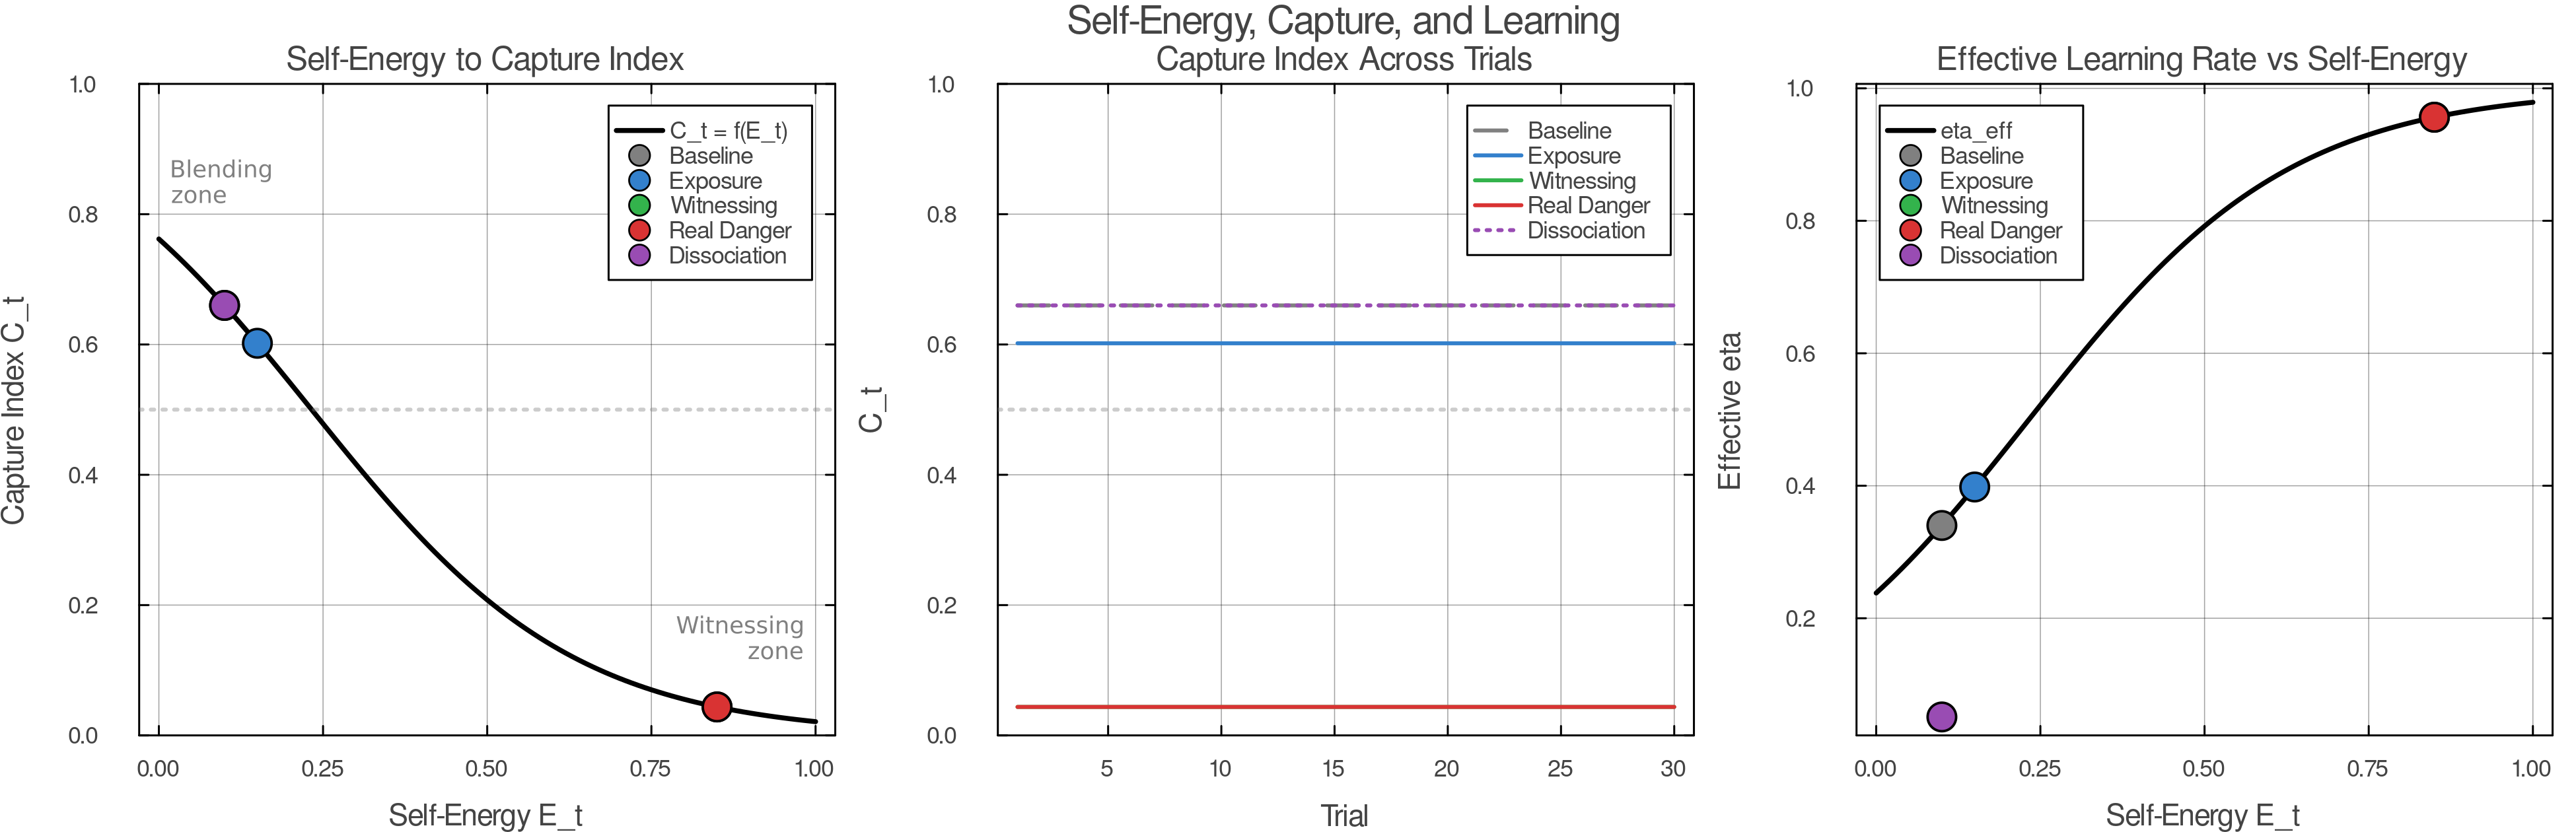
\includegraphics[width=0.96\linewidth]{fig5_capture_index.png}
\caption{Capture index as a function of effective part-bundle precision and present-context evidence precision. High Self-energy lowers capture by reducing effective part dominance while amplifying context weighting.}
\label{fig:capture-index}
\end{figure}

When Self-energy is low and a part activates, the part's high-precision
priors dominate inference. Its beliefs about self-state (``I am
small''), world-state (``this is dangerous''), policy (``I must
avoid''), and expected outcome (``avoidance keeps me safe'') organize
ongoing inference and action selection. Present-context evidence --- the
therapist's voice, the safety of the room, the fact of inhabiting an
adult body --- goes functionally offline. The sensory channels remain
intact, but the part's precision so outweighs context precision that
incoming signals exert little influence on inference.

This is what IFS clinicians call blending. Phenomenologically, blending
is the difference between having a feeling and being organized by it.
The part's beliefs do not present as beliefs; they present as reality.
``I am afraid'' is not a report about an internal state; it is the only
available description of the world.

Formally, blending corresponds to the regime where the capture index

\[C_t = \frac{\pi_{\text{part}}^{\text{eff}}}{\pi_{\text{part}}^{\text{eff}} + \lambda_{\text{ctx}}^{\text{eff}}}\]

approaches 1. Here
\(\pi_{\text{part}}^{\text{eff}} = r_t \cdot \pi_{\text{part}} \cdot e^{-\beta E_t}\)
is the effective precision of the active part bundle, modulated by
activation strength \(r_t\) and Self-energy \(E_t\), while
\(\lambda_{\text{ctx}}^{\text{eff}} = \lambda_{\text{ctx}} \cdot e^{+\gamma E_t}\)
is the effective precision on present-context evidence. When \(E_t\) is
low, both exponential terms are near 1, and the part's high base
precision \(\pi_{\text{part}}\) overwhelms context.

Blending is not all-or-none. The capture index is continuous, and the
degree of blending varies with the strength of activation, the rigidity
of the part's priors, and the momentary level of Self-energy.
Clinically, there are thresholds that matter --- particularly whether
the system retains enough context precision to sustain dual awareness,
the capacity to register both the part's perspective and the present
situation simultaneously. Below that threshold, the part's beliefs
function as identity rather than content. Above it, they can begin to be
held as object.

Blending is also self-reinforcing: once a part captures inference, its
predictions bias sampling and interpretation in ways that appear to
confirm the part's own model. The world looks dangerous because the
system is sampling through a danger filter, and the apparent
confirmation increases precision on the danger prior further. Breaking
this cycle typically requires some form of external perturbation --- a
therapist's question, a shift in bodily state, a moment of unexpected
safety that the part's filter cannot entirely suppress.

\subsection{8.2 Witnessing}\label{witnessing}

Consider the same part activating under high Self-energy. The bundle
still fires and heart rate still rises. The learned associations between
cue and threat come online. But this time, present-context evidence
remains strongly weighted: the room is safe, the therapist is present,
and the body is adult rather than six years old.

The same activation now produces a different inferential regime. The
capture index \(C_t\) stays well below 1, not because the part is less
active --- \(r_t\) may be equally high --- but because Self-energy has
shifted the precision balance. The exponential scaling
\(e^{-\beta E_t}\) reduces the effective dominance of the part's priors,
while \(e^{+\gamma E_t}\) amplifies the weight of context evidence. The
part's beliefs are now active contributors to inference, not its sole
determinants.

This is witnessing. Phenomenologically, it is ``a part of me is afraid''
--- the same activation, held in a different relation. The fear is
present, perhaps intensely so, yet it is present \emph{to} an observing
subject rather than constituting the whole subject.

Witnessing is formally distinct from distraction or dissociation because
the part remains active. The system has not suppressed activation or
numbed context; it has altered the inferential regime in which
activation occurs. The part's priors are live --- generating
predictions, producing prediction errors, and competing for influence on
policy selection --- but they are competing in a regime where context
evidence has enough weight to prevent capture. That distinction matters
because only active priors confronted by intact context can be revised.

This distinction matters because it explains why not all forms of
``calming down'' are therapeutically equivalent. A person who distracts
themselves from a triggered part (watches television, changes the
subject, intellectualizes) may reduce the capture index to near zero ---
but they do so by reducing \(r_t\), not by maintaining activation under
high Self-energy. The part's priors go dormant. Nothing is live to
revise. A person who dissociates may appear calm, but dissociation
achieves its quiet by reducing precision on sensory evidence
(\(\lambda_{\text{ctx}}\) drops), not by maintaining context. The part
may remain partially active, but context is offline, so the conditions
for revision are not met.

Witnessing is the specific configuration in which activation stays high
and context stays online. It is the only regime that satisfies both
conditions for durable revision simultaneously.

\subsection{8.3 The 2x2: Part Activation and
Self-Energy}\label{the-2x2-part-activation-and-self-energy}

The relationship between blending and witnessing can be clarified by a
simple matrix crossing two continuous dimensions: the activation
strength of a part (\(r_t\)) and the degree of Self-energy (\(E_t\)).

\begin{table}[htbp]
\centering
\small
\begin{tabular}{|p{0.28\linewidth}|p{0.28\linewidth}|p{0.28\linewidth}|}
\hline
 & \textbf{Low Self-energy ($E_t$)} & \textbf{High Self-energy ($E_t$)} \\
\hline
\textbf{Low part activation} & Baseline / ordinary cognition & Presence / Self \\
\hline
\textbf{High part activation} & Blending & Witnessing (therapeutic zone) \\
\hline
\end{tabular}
\end{table}

The lower-left cell is familiar: a triggered part dominates, and the
person is blended. The upper-right cell is also recognizable: no part is
strongly active, and the person is in a Self-led state --- open,
curious, grounded. The upper-left is ordinary life: no particular part
activated, no particular depth of presence.

The therapeutic zone is the lower-right: high part activation
co-occurring with high Self-energy. This is the cell that IFS therapy
specifically targets. It requires the clinician to help the client
activate a part --- invite it forward, ask about it, explore its beliefs
--- while simultaneously maintaining enough Self-energy that the
activation does not become capture. The therapist's regulated presence
often scaffolds this balance, supplying external support for Self-energy
(\(u_t\) in the simulation) until the client's own capacity stabilizes.

The matrix makes visible why therapy is difficult: the therapeutic cell
requires simultaneous conditions that naturally oppose each other. Part
activation tends to reduce Self-energy (the fear itself is
dysregulating), while high Self-energy tends to keep parts from
activating fully (the system is less reactive). Skilled therapeutic work
navigates this tension, titrating activation to stay in the witnessing
zone without tipping into blending.

\subsection{8.4 The Clinical Probe}\label{the-clinical-probe}

In practice, clinicians assess the shift from blending to witnessing not
by measuring activation levels or Self-energy directly but by observing
the quality of the client's relationship to the activated part. The
canonical IFS probe is: ``How do you feel toward this part?''

If the client responds with the part's own affect --- ``I'm terrified,''
``I hate it,'' ``I need to get away'' --- the system is likely blended.
The part's beliefs are operating as identity, and the response comes
from inside the part's inferential regime.

If the client responds with one of the qualities associated with Self
--- curiosity, compassion, openness, calm interest --- the system is
likely witnessing. The part is active, but the response comes from
outside the part's capture. The client can relate \emph{to} the part
rather than \emph{as} the part.

The probe can be read as a real-time assay of the capture index.
Responses marked by curiosity, compassion, or calm suggest \(C_t\) is
low enough that context-informed inference is generating the relational
stance. Responses that speak from the part itself --- ``I'm terrified,''
``I need to get away'' --- suggest \(C_t\) is high enough that the
part's own priors are producing the reply. The probe does not measure
activation; it measures the relationship to activation, which is
precisely the variable the model identifies as decisive.

\subsection{8.5 Why the Distinction
Matters}\label{why-the-distinction-matters}

In IFS, the central therapeutic question is not whether a part
activates. Activation is necessary --- without it, there is nothing live
to revise. The question is whether activation unfolds under capture or
in context.

Under capture, the part may activate thousands of times across a
person's life, each time producing the same fear, the same avoidance,
the same self-assessment --- and each time confirming its own
predictions within its own closed loop. Present reality has been
functionally excluded from inference; the system cannot register the
mismatch between the part's outdated priors and current conditions.

Under context, the same activation becomes an opportunity for revision.
The mismatch between ``I am six and helpless'' and ``I am thirty and
sitting in a safe room'' is computationally available. The conditions
for updating are met.

This is the answer to the first half of the paper's central question:
what determines whether a part takes over or can be held in context?
Self-energy largely determines which regime obtains, and thus whether
activation will merely repeat a prior or expose it to revision. The next
section addresses the second half: why only the witnessing regime
permits lasting change.

\section{9. Why Only Witnessing Permits Lasting
Change}\label{why-only-witnessing-permits-lasting-change}

The previous section established that Self-energy determines whether
part activation becomes capture or context-held awareness. This section
addresses the deeper question: why does only the witnessing regime
produce durable revision of the part's outdated beliefs?

\subsection{9.1 The Three Conditions}\label{the-three-conditions}

Durable change requires three conditions to hold simultaneously:

\begin{enumerate}
\def\labelenumi{\arabic{enumi}.}
\item
  \textbf{The part must be active.} Its priors must be live ---
  generating predictions, influencing inference, producing the
  phenomenology of the original experience. Without activation, there is
  nothing to revise. The target beliefs are dormant, and no amount of
  safety or insight can reach them.
\item
  \textbf{Present-context evidence must be online.} The system must have
  access to information that contradicts the part's outdated priors ---
  the fact of being adult, the safety of the current environment, the
  availability of resources the original situation lacked. Without
  context, there is nothing to revise \emph{with}.
\item
  \textbf{Self-energy must be high enough to prevent capture.} The
  part's activation must not dominate inference to the point where
  context is excluded. If the part captures the system, conditions 1 and
  2 cannot coexist: the part is active, but context has been
  functionally excluded.
\end{enumerate}

Each condition alone is insufficient. Conditions 1 and 2 without
condition 3 produce blending --- the part is active and context
nominally exists, but the part's precision overwhelms context. Condition
2 without condition 1 produces ordinary calm --- the person feels safe
but the part's priors are not engaged and cannot be updated. Conditions
1 and 3 without condition 2 would require activation under high
Self-energy in the absence of corrective evidence --- a theoretically
possible but clinically unusual configuration.

Witnessing is the regime in which all three conditions are satisfied. It
is not a technique but an inferential configuration: the part's priors
are active and generating predictions, context evidence is weighted
heavily enough to produce prediction errors against those priors, and
Self-energy prevents the part from suppressing the resulting mismatch
signal.

\subsection{9.2 Why Blending Blocks
Revision}\label{why-blending-blocks-revision}

Under blending, the part's priors dominate inference so thoroughly that
contradicting evidence cannot gain computational traction. The
prediction error that would ordinarily drive updating --- ``your prior
says danger, but the evidence says safety'' --- is attenuated by the
precision imbalance. The part's model is internally consistent: it
predicts danger, samples for danger cues, finds what looks like danger
(through the filter of its own expectations), and confirms its own
predictions. The system is trapped in what amounts to a local minimum of
free energy --- a stable configuration that resists perturbation because
the part's high precision means the cost of revising its beliefs exceeds
the cost of discounting the evidence.

This is why a part can activate thousands of times across a lifetime
without updating. Each activation occurs under the same precision regime
that formed the part in the first place. The experience of being
triggered is familiar precisely because nothing new is being learned.

\subsection{9.3 Why Calm Without Activation Is
Insufficient}\label{why-calm-without-activation-is-insufficient}

A person can be entirely calm, grounded, and Self-led --- high \(E_t\),
low \(r_t\) --- and yet the part's outdated beliefs remain untouched.
The priors are dormant. They are not generating predictions, not
producing prediction errors, not competing with context. The system is
in the upper-right cell of the 2x2 matrix: presence without therapeutic
engagement.

This is why insight alone rarely produces lasting change. A person may
understand intellectually that their fear of dogs is outdated, that they
are no longer six years old, that the original danger has passed. This
understanding exists in context, but it does not reach the part because
the part is not active. The understanding and the outdated belief occupy
different inferential regimes and never meet.

IFS therapy is distinctive precisely because it deliberately activates
the part --- invites it forward, asks about its beliefs, engages its
phenomenology --- while maintaining the Self-energy needed to prevent
that activation from becoming capture. The therapeutic action is not
activation alone (that happens in every triggering event) and not calm
alone (that happens in meditation), but their co-occurrence under
conditions of non-capture.

\subsection{9.4 Unburdening as Upstream Prior
Revision}\label{unburdening-as-upstream-prior-revision}

In IFS clinical language, the durable change that occurs under
witnessing is called \emph{unburdening}. The present model interprets
unburdening as revision of the part's upstream priors --- specifically,
the self-state and world-state beliefs that sit at the top of the part's
causal chain.

A part bundles priors in a causal sequence: self-state (``I am six and
helpless'') conditions capability assessment (``I cannot protect
myself''), which conditions threat meaning (``this is dangerous to
me''), which conditions policy (``I must avoid''). Under the H1 model
proposed in this paper, witnessing revises the upstream priors first.
The system infers ``I am adult and capable,'' and that revision cascades
downstream: the threat becomes reassessable, and avoidance is no longer
the only viable policy.

This causal ordering explains a clinical observation that is otherwise
puzzling: why does IFS unburdening often feel sudden? The part has been
carrying the same beliefs for years or decades, and then in a single
session --- sometimes in a single moment --- the beliefs shift. The
model suggests this is not sudden learning from accumulated evidence but
a threshold effect: once the upstream prior (self-state) revises under
witnessing, the downstream beliefs that depended on it are no longer
supported and can update rapidly.

\subsection{9.5 Partial Revision}\label{partial-revision}

The model predicts that revision can be partial. If activation is
present and context is online but the witnessing window is brief or
unstable --- if Self-energy fluctuates, or the client slips in and out
of blending --- upstream priors may soften without fully revising. The
part's beliefs become less rigid, less dominant, but not yet fully
updated.

Clinically, this corresponds to burdens that lighten without fully
releasing. The client reports that the fear is ``less intense'' or
``further away'' but not gone. The part still activates in response to
the old cues, but with lower precision and less capture. In IFS
practice, the repeated question ``Is there more?'' reflects this
possibility: full unburdening may require sustained or repeated
witnessing, not a single brief contact.

Formally, partial revision occurs when the prediction errors generated
during witnessing are sufficient to reduce the concentration parameters
of the part's Dirichlet priors but not to shift their modes. The beliefs
soften --- become less certain --- without yet converging on the new
context-consistent values. This intermediate state is neither the
original rigid bundle nor a fully revised one, and it predicts a
characteristic clinical trajectory: gradual loosening across sessions,
punctuated by moments of deeper revision when witnessing is sustained.

\subsection{9.6 The Exposure Comparison}\label{the-exposure-comparison}

The distinction between witnessing and exposure therapy is not that one
works and the other does not. Exposure therapy produces real clinical
gains. The model's claim is that the mechanisms differ, and the
differences explain observed patterns in speed, depth, and
generalization of change.

In exposure therapy, the client confronts the feared stimulus under
conditions of activation. Context evidence is present --- the therapy
room is safe, the exposure is controlled --- but Self-energy is not
specifically elevated. The client is activated and in contact with
corrective evidence, but the part's priors may retain high effective
precision. Learning occurs, but it occurs primarily at the level of
threat meaning: the specific stimulus is reclassified from dangerous to
safe. Self-state priors (``I am helpless'') may shift weakly or not at
all.

Under witnessing, the same corrective evidence is available, but
Self-energy shifts the precision balance. The part's priors lose
effective dominance, allowing evidence to reach upstream beliefs ---
including self-state. Because self-state is upstream of threat meaning
in the H1 model, revising ``I am helpless'' to ``I am capable'' cascades
to threat reassessment more broadly than revising a single
stimulus-threat association.

This predicts that witnessing should produce broader generalization than
exposure. Exposure retrains ``this dog is safe''; witnessing retrains
``I am someone who can handle dogs.'' The first is stimulus-specific;
the second transfers to novel stimuli that share the underlying
self-state prior.

\section{10. Protectors}\label{protectors}

In IFS clinical work, parts are not encountered in isolation. Before a
client can access an exile --- a part carrying the original wound ---
they typically encounter protectors: parts whose function is to prevent
the exile's activation from destabilizing the system.

\subsection{10.1 Protectors as Policy
Priors}\label{protectors-as-policy-priors}

The present model formalizes protectors minimally, as policy priors
combined with access-control tendencies. A protector is a learned
pattern that biases action selection toward avoidance, distraction,
numbing, or preemptive management whenever cues approach the exile's
activation threshold. In the model's terms, a protector increases the
prior probability of policies that reduce \(r_t\) --- keeping the
exile's activation low and thereby preventing blending.

This is locally rational behavior. If exile takeover has repeatedly been
overwhelming --- if blending with the exile produces intolerable
distress, functional impairment, or further traumatization --- then
cautious gatekeeping is not pathology from the protector's point of
view. It is optimized prevention, given the system's history and the
system's assessment of available Self-energy.

\subsection{10.2 Managers and
Firefighters}\label{managers-and-firefighters}

IFS distinguishes two classes of protectors. \emph{Managers} operate
proactively, planning trajectories through state space that avoid
exile-activating regions. They maintain control, anticipate threats, and
organize daily life to minimize triggering. In active inference terms,
managers are policy priors with high temporal depth --- they plan ahead
to keep the system away from dangerous states.

\emph{Firefighters} operate reactively. When a trigger slips through the
manager's defenses and the exile begins to activate, firefighters
rapidly minimize acute distress through impulsive action: substance use,
dissociation, rage, binge eating, self-harm. In the model's terms,
firefighters are policy priors with low temporal depth --- they minimize
immediate free energy without regard for long-term consequences.

\subsection{10.3 What the Model Does Not Yet
Capture}\label{what-the-model-does-not-yet-capture}

The present model formalizes only the minimum protector function:
preventing destabilizing takeover. It does not yet model the full
clinical richness of protectors, including trust assessment, conditional
permission, role transformation after unburdening, and the distinct
strategic styles that differentiate manager and firefighter
configurations.

In clinical practice, protectors are not merely policies to be
overridden. They have their own trust conditions: a protector may step
back only when it assesses that Self-energy is sufficient, that the
therapeutic context is safe, and that the exile's activation will not
overwhelm the system. This trust assessment is a sophisticated
computation that the current model represents only implicitly, through
the dependence of the capture index on Self-energy. A more complete
model would formalize protector trust as an explicit variable
conditioning the gate on exile access.

\section{11. Multi-Part Polarization}\label{multi-part-polarization}

The model presented so far addresses single-part dynamics: one part
activating, blending or witnessing, and potentially revising. Clinical
systems are rarely so simple. One of the most recognizable phenomena in
IFS practice is \emph{polarization}: the experience of being pulled in
opposite directions by competing parts.

\subsection{11.1 Polarization as Mutual Threat
Modeling}\label{polarization-as-mutual-threat-modeling}

Polarization occurs when two or more part-bundles assign high expected
danger to each other's preferred policies. Consider a system with two
activated parts:

\begin{itemize}
\tightlist
\item
  \textbf{Part A} (attachment-seeking): priors favoring approach,
  disclosure, and connection. Expected outcome of Part B's policy:
  abandonment and isolation.
\item
  \textbf{Part B} (self-protective): priors favoring withdrawal,
  guardedness, and avoidance. Expected outcome of Part A's policy:
  vulnerability and harm.
\end{itemize}

Each part treats the other's preferred action as dangerous. When Part A
gains influence and the system begins to approach, Part B's threat
estimate rises, increasing its activation and pulling the system back.
When Part B dominates and the system withdraws, Part A's threat estimate
rises --- loneliness and disconnection feel intolerable --- and pulls
the system forward again.

\subsection{11.2 Phenomenology}\label{phenomenology}

Under low Self-energy, this mutual threat modeling produces a
characteristic phenomenology:

\begin{itemize}
\tightlist
\item
  \textbf{Oscillation:} rapid reversals between incompatible action
  tendencies.
\item
  \textbf{Ambivalence:} the subjective sense of wanting and not-wanting
  simultaneously.
\item
  \textbf{Each side feeling fully true when active:} during Part A's
  capture, approach feels essential and withdrawal feels cowardly.
  During Part B's capture, withdrawal feels essential and approach feels
  reckless.
\item
  \textbf{Exhaustion:} the metabolic and psychological cost of unstable
  agency --- energy spent switching between regimes without settling
  into either.
\item
  \textbf{Chronic indecision:} the system cannot commit to a stable
  policy because each commitment triggers the opposing part.
\end{itemize}

\subsection{11.3 Self-Energy and
De-Polarization}\label{self-energy-and-de-polarization}

Higher Self-energy dampens polarization dynamics. When \(E_t\) is
elevated, neither part can fully capture inference. Both perspectives
remain active without either dominating. The system can hold ``I want
connection'' and ``I need to protect myself'' simultaneously, as objects
of awareness rather than competing identities.

This is the precondition for what IFS clinicians call negotiation or
de-polarization: the emergence of policies that honor both parts'
concerns. In the model's terms, high Self-energy reduces the effective
precision of both part-bundles, increasing policy entropy and allowing
mixed or negotiated actions to emerge.

Although the appendix formalizes polarization as a two-bundle system,
clinical systems often contain larger polarization networks in which
multiple protectors and exiles mutually recruit one another across
several steps. The two-bundle model captures the core mechanism;
extending it to multi-part networks is a direction for future work.

The main text provides the mechanistic account; Appendix B provides the
companion simulation.

\section{12. Main Simulation}\label{main-simulation}

\subsection{12.1 Purpose}\label{purpose}

The simulation tests the paper's central claim in a minimal case: the
same part activates under different levels of Self-energy, yielding
either blending or witnessing. The question is whether only the
witnessing regime produces durable updating of the part's outdated
priors.

A secondary purpose is to compare two causal structures:

\begin{itemize}
\tightlist
\item
  \textbf{H1 (self-state-upstream):} self-state is causally upstream of
  threat meaning. Witnessing revises ``who I am'' first, and threat
  reassessment follows.
\item
  \textbf{H2 (threat-primary):} threat meaning is primary. The system
  reinterprets the threat first, and self-state follows.
\end{itemize}

\subsection{12.2 Design Principles}\label{design-principles}

The simulation is designed so that the comparison between conditions is
fair:

\begin{itemize}
\tightlist
\item
  Exposure and witnessing are implemented over the same task structure,
  the same cue channels, and the same part-activation pathway. The
  manipulated difference is the inferential regime governed by
  Self-energy.
\item
  The central comparison is meaningful only if part activation (\(r_t\))
  remains comparable across conditions, allowing the simulations to
  isolate the relation-to-activation rather than activation magnitude
  itself.
\item
  Witnessing is not given special channels or information unavailable to
  exposure. The difference is inferential regime, not model
  architecture.
\end{itemize}

\subsection{12.3 Architecture}\label{architecture}

The simulation uses a discrete POMDP with three hidden factors:

\begin{enumerate}
\def\labelenumi{\arabic{enumi}.}
\tightlist
\item
  \textbf{External context} \(c \in \{\text{safe}, \text{dangerous}\}\)
\item
  \textbf{Self-state}
  \(s \in \{\text{child\_helpless}, \text{adult\_capable}\}\)
\item
  \textbf{Threat meaning} \(m \in \{\text{danger}, \text{safe}\}\)
\end{enumerate}

Four observation modalities:

\begin{enumerate}
\def\labelenumi{\arabic{enumi}.}
\tightlist
\item
  \textbf{External cue}
  \(o_{\text{ext}} \in \{\text{ambiguous}, \text{clear\_safe}, \text{clear\_threat}\}\)
\item
  \textbf{Interoceptive arousal}
  \(o_{\text{int}} \in \{\text{calm}, \text{activated}, \text{panic}\}\)
\item
  \textbf{Outcome}
  \(o_{\text{out}} \in \{\text{relief}, \text{neutral}, \text{harm}\}\)
\item
  \textbf{Present-context support}
  \(o_{\text{ctx}} \in \{\text{alone\_overwhelmed}, \text{supported\_here\_now}\}\)
\end{enumerate}

Three policies: \(\pi_{\text{avoid}}\) (fast disengagement),
\(\pi_{\text{inspect}}\) (approach and sample), \(\pi_{\text{stay}}\)
(maintain contact).

The part bundle is represented as strong priors on
\(s = \text{child\_helpless}\), \(m = \text{danger}\), and
\(\pi_{\text{avoid}}\).

\subsection{12.4 Self-Energy
Implementation}\label{self-energy-implementation}

Self-energy \(E_t \in [0,1]\) modulates effective precisions:

\[\pi_{\text{part}}^{\text{eff}} = r_t \cdot \pi_{\text{part}} \cdot e^{-\beta E_t}\]
\[\lambda_{\text{ctx}}^{\text{eff}} = \lambda_{\text{ctx}} \cdot e^{+\gamma E_t}\]

An optional external support parameter \(u_t\) allows Self-energy
dynamics:

\[E_{t+1} = \text{clip}(E_t + u_t + \alpha W_t - \beta' B_t,\ 0,\ 1)\]

where \(W_t\) indexes successful witnessing episodes and \(B_t\) indexes
blending episodes, capturing the clinical observation that successful
witnessing strengthens Self-energy while blending episodes can erode it.

\subsection{12.5 Conditions}\label{conditions}

\begin{figure}[htbp]
\centering
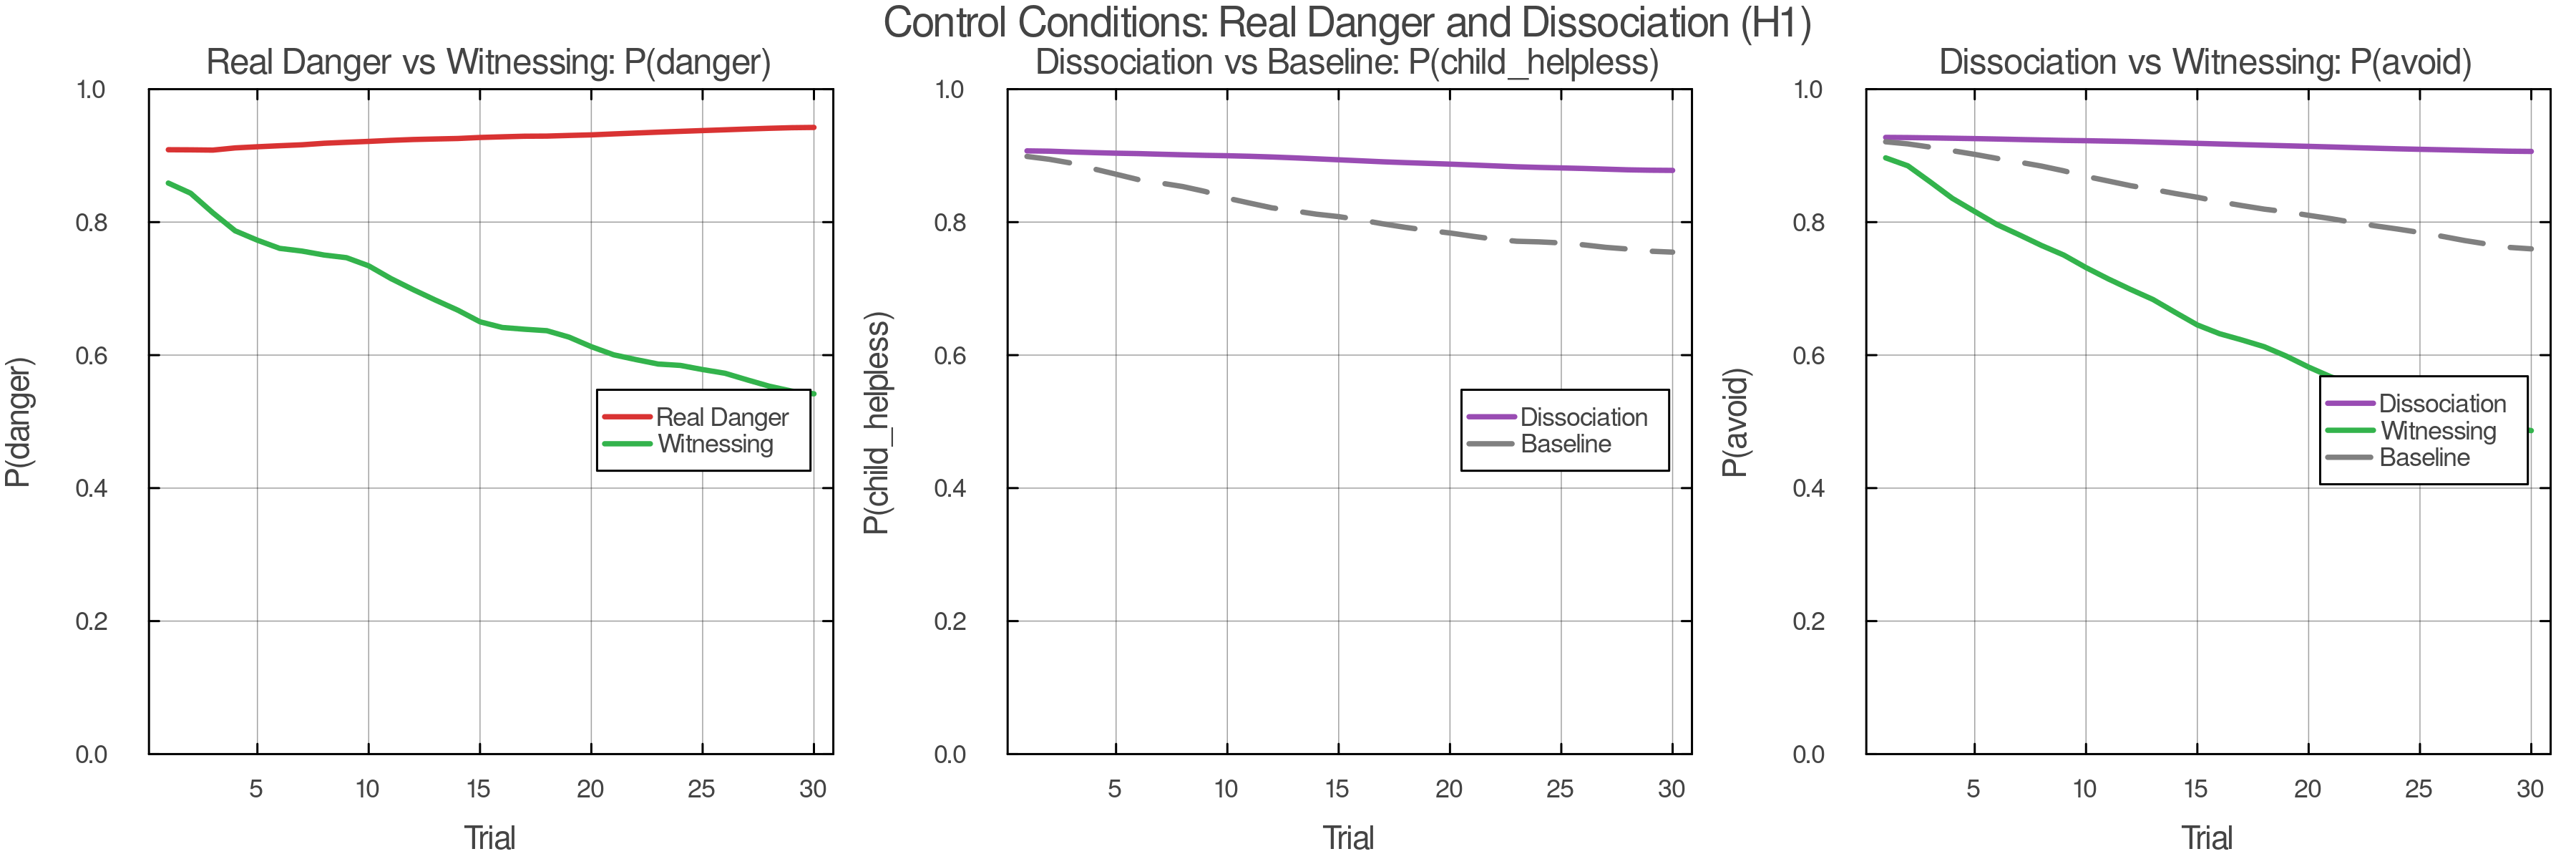
\includegraphics[width=0.96\linewidth]{fig4_control_conditions.png}
\caption{Control conditions for the main simulation. The critical comparison holds task structure constant while varying the inferential regime through Self-energy.}
\label{fig:control-conditions}
\end{figure}

Five conditions test the model's predictions:

\textbf{Condition 1 (Baseline):} Safe world, ambiguous cue, low \(E_t\),
free policy selection. Predicted: high capture, high avoidance, minimal
updating.

\textbf{Condition 2 (Exposure):} Same safe world and ambiguous cue.
\(E_t\) held low (same as baseline). Policy constrained to inspect/stay
--- forced contact with the stimulus. Predicted: some threat updating,
weaker self-state revision, slower and narrower change.

\textbf{Condition 3 (Witnessing):} Same safe world, ambiguous cue, same
forced contact as exposure. \(E_t\) elevated. Predicted: same
activation, different relationship; part held in context; earlier
self-state revision; downstream threat revision; broader generalization.

\textbf{Condition 4 (Real-danger control):} Dangerous world, \(E_t\)
elevated. Predicted: adaptive fear remains. The model does not predict
indiscriminate calm.

\textbf{Condition 5 (Dissociation control):} Safe world, part activation
present, low \(E_t\), reduced context-evidence precision. Predicted:
disturbance may drop, but durable updating remains poor. Distinguishes
witnessing from numbed disengagement.

\subsection{12.6 H1 vs.~H2}\label{h1-vs.-h2}

Under \textbf{H1 (self-state-upstream):} \(o_{\text{ctx}}\) primarily
informs \(s\); \(s\) strongly conditions \(m\); \(m\) conditions policy.
Witnessing should produce: \(P(s = \text{adult\_capable})\) rises first,
\(P(m = \text{safe})\) follows, \(P(\text{avoid})\) falls last.

Under \textbf{H2 (threat-primary):} \(o_{\text{ext}}\) and
\(o_{\text{int}}\) primarily inform \(m\); \(m\) then influences \(s\).
Exposure and witnessing should look more similar; the generalization
advantage of witnessing should shrink.

\section{13. Results and Expected
Signatures}\label{results-and-expected-signatures}

This section states the model's predicted signatures. Final simulation
results will determine whether these predictions are confirmed.

\subsection{13.1 Same Activation, Different
Relationship}\label{same-activation-different-relationship}

For matched part activation \(r_t\) across conditions, low Self-energy
should produce blending-like capture (high \(C_t\), avoidant policy,
minimal revision) while high Self-energy should produce witnessing-like
context holding (low \(C_t\), exploratory policy, active revision). The
capture index provides a direct phenomenological readout:
\(C_t > \theta_{\text{high}}\) corresponds to ``I am afraid'';
\(C_t < \theta_{\text{low}}\) with \(r_t\) still elevated corresponds to
``a part of me is afraid.''

\subsection{13.2 Order of Revision Under
H1}\label{order-of-revision-under-h1}

\begin{figure}[htbp]
\centering
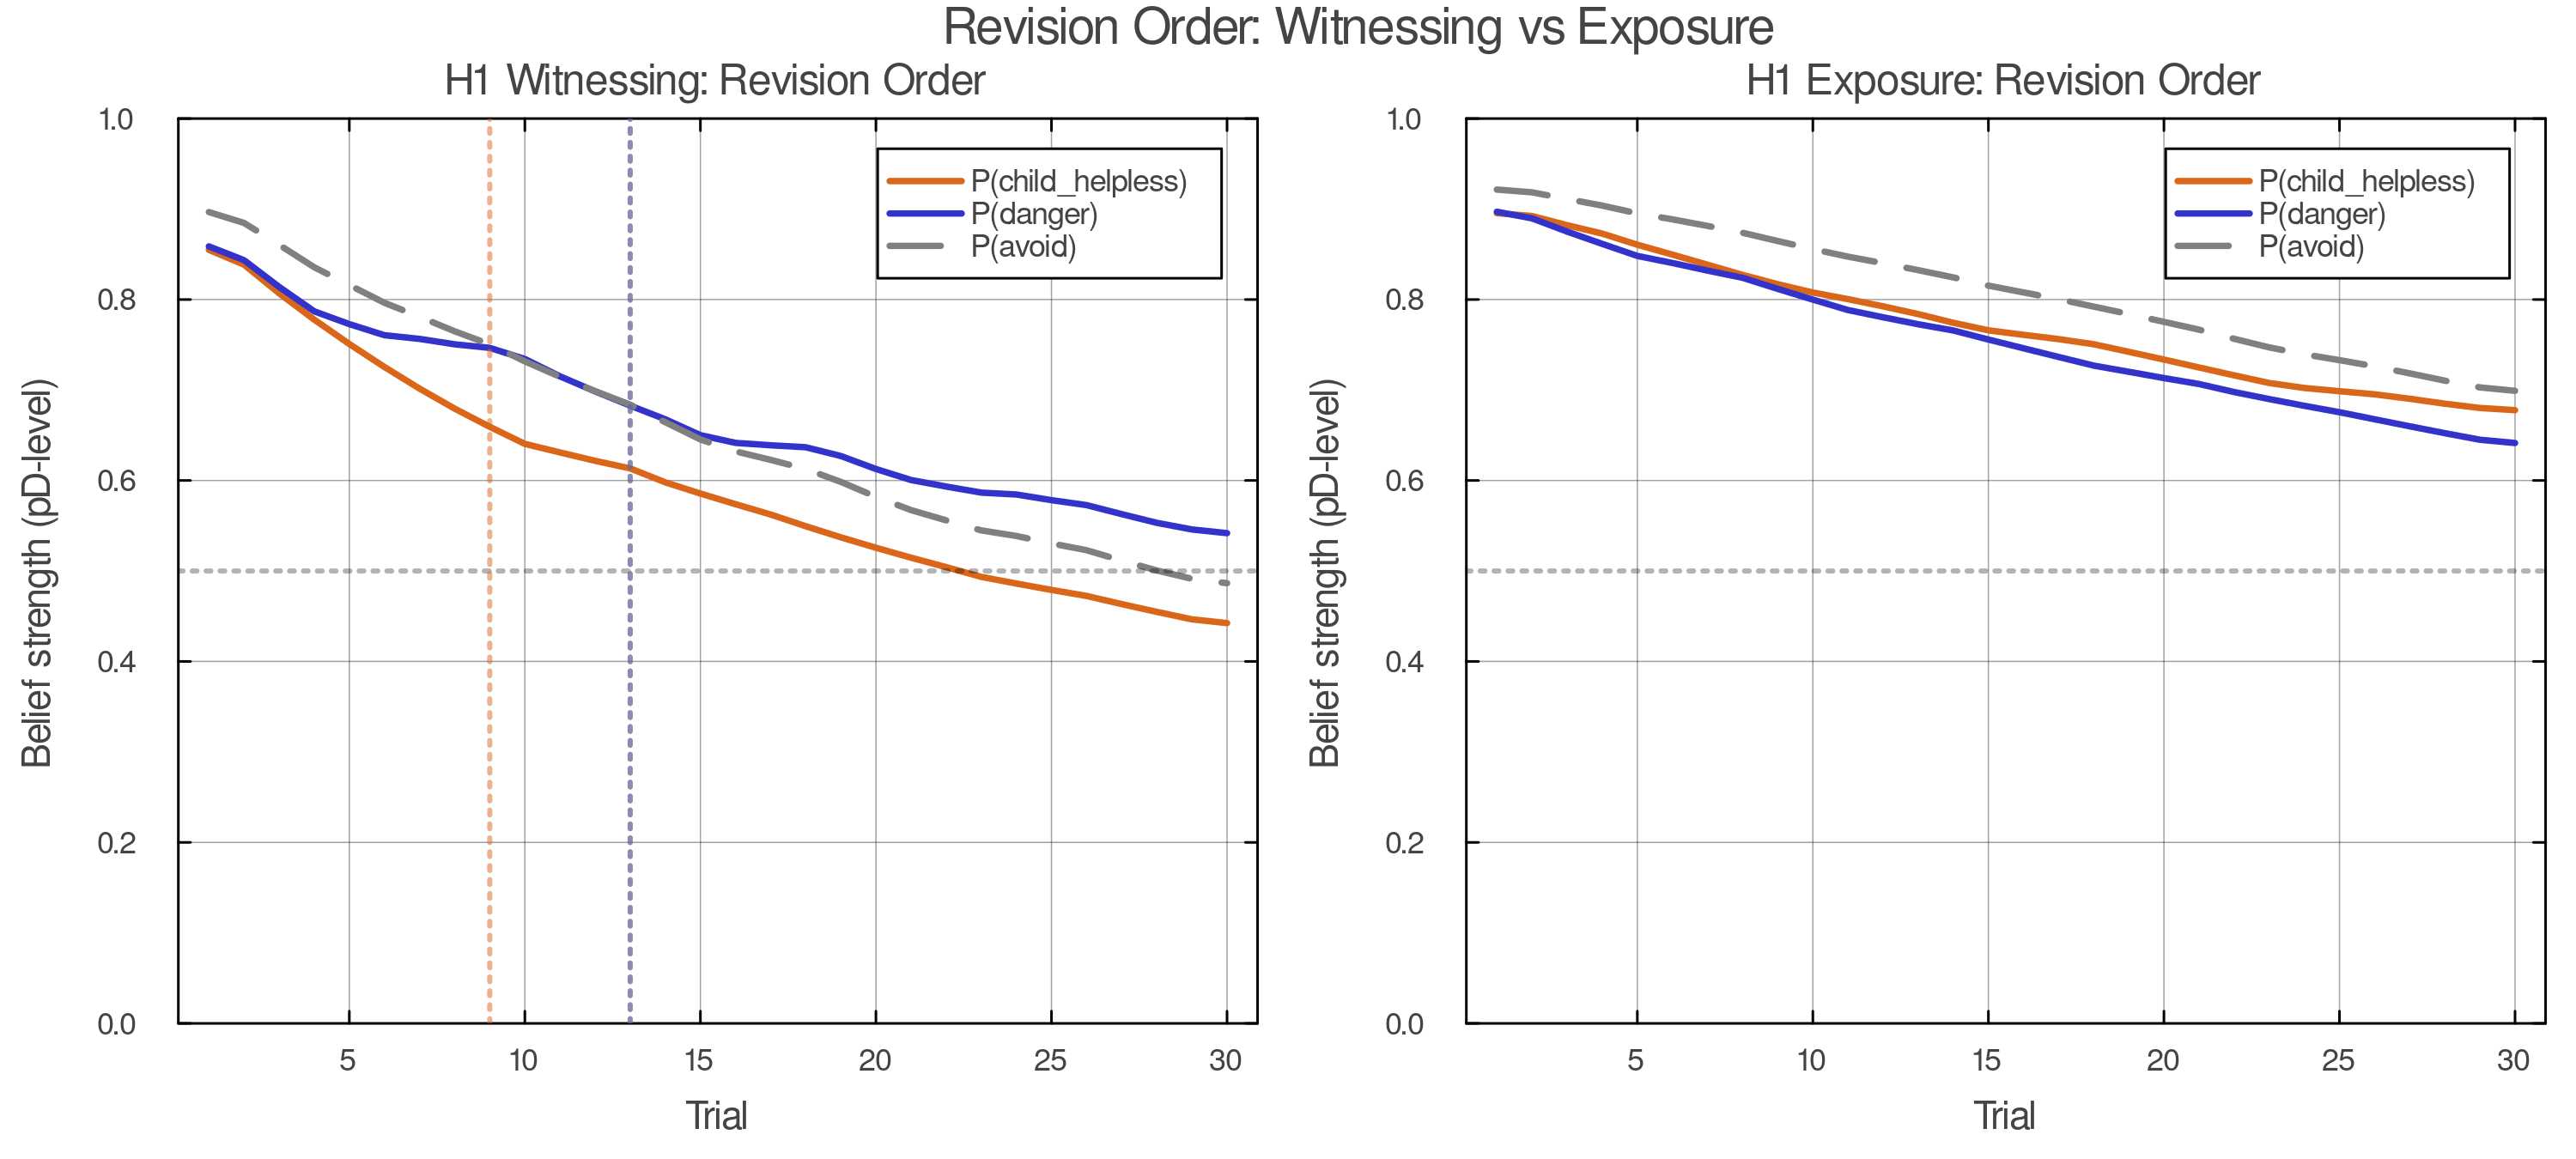
\includegraphics[width=0.96\linewidth]{fig6_revision_order.png}
\caption{Expected order of revision under H1: self-state shifts first, threat meaning follows, and policy relaxation lags both.}
\label{fig:revision-order}
\end{figure}

Under witnessing in the H1 model, revision should follow a temporal
ordering:

\begin{enumerate}
\def\labelenumi{\arabic{enumi}.}
\tightlist
\item
  \(P(s = \text{adult\_capable})\) rises first (self-state revision)
\item
  \(P(m = \text{safe})\) rises second (threat reassessment)
\item
  \(P(\text{avoid})\) falls third (policy relaxation)
\end{enumerate}

This ordering is a strong prediction of the self-state-upstream
hypothesis. It corresponds to the clinical observation that protectors
relax downstream of upstream revision --- the system stops avoiding not
because it has been convinced that this particular stimulus is safe, but
because it no longer experiences itself as helpless in the face of
threat.

\subsection{13.3 Exposure Comparison}\label{exposure-comparison}

\begin{figure}[htbp]
\centering
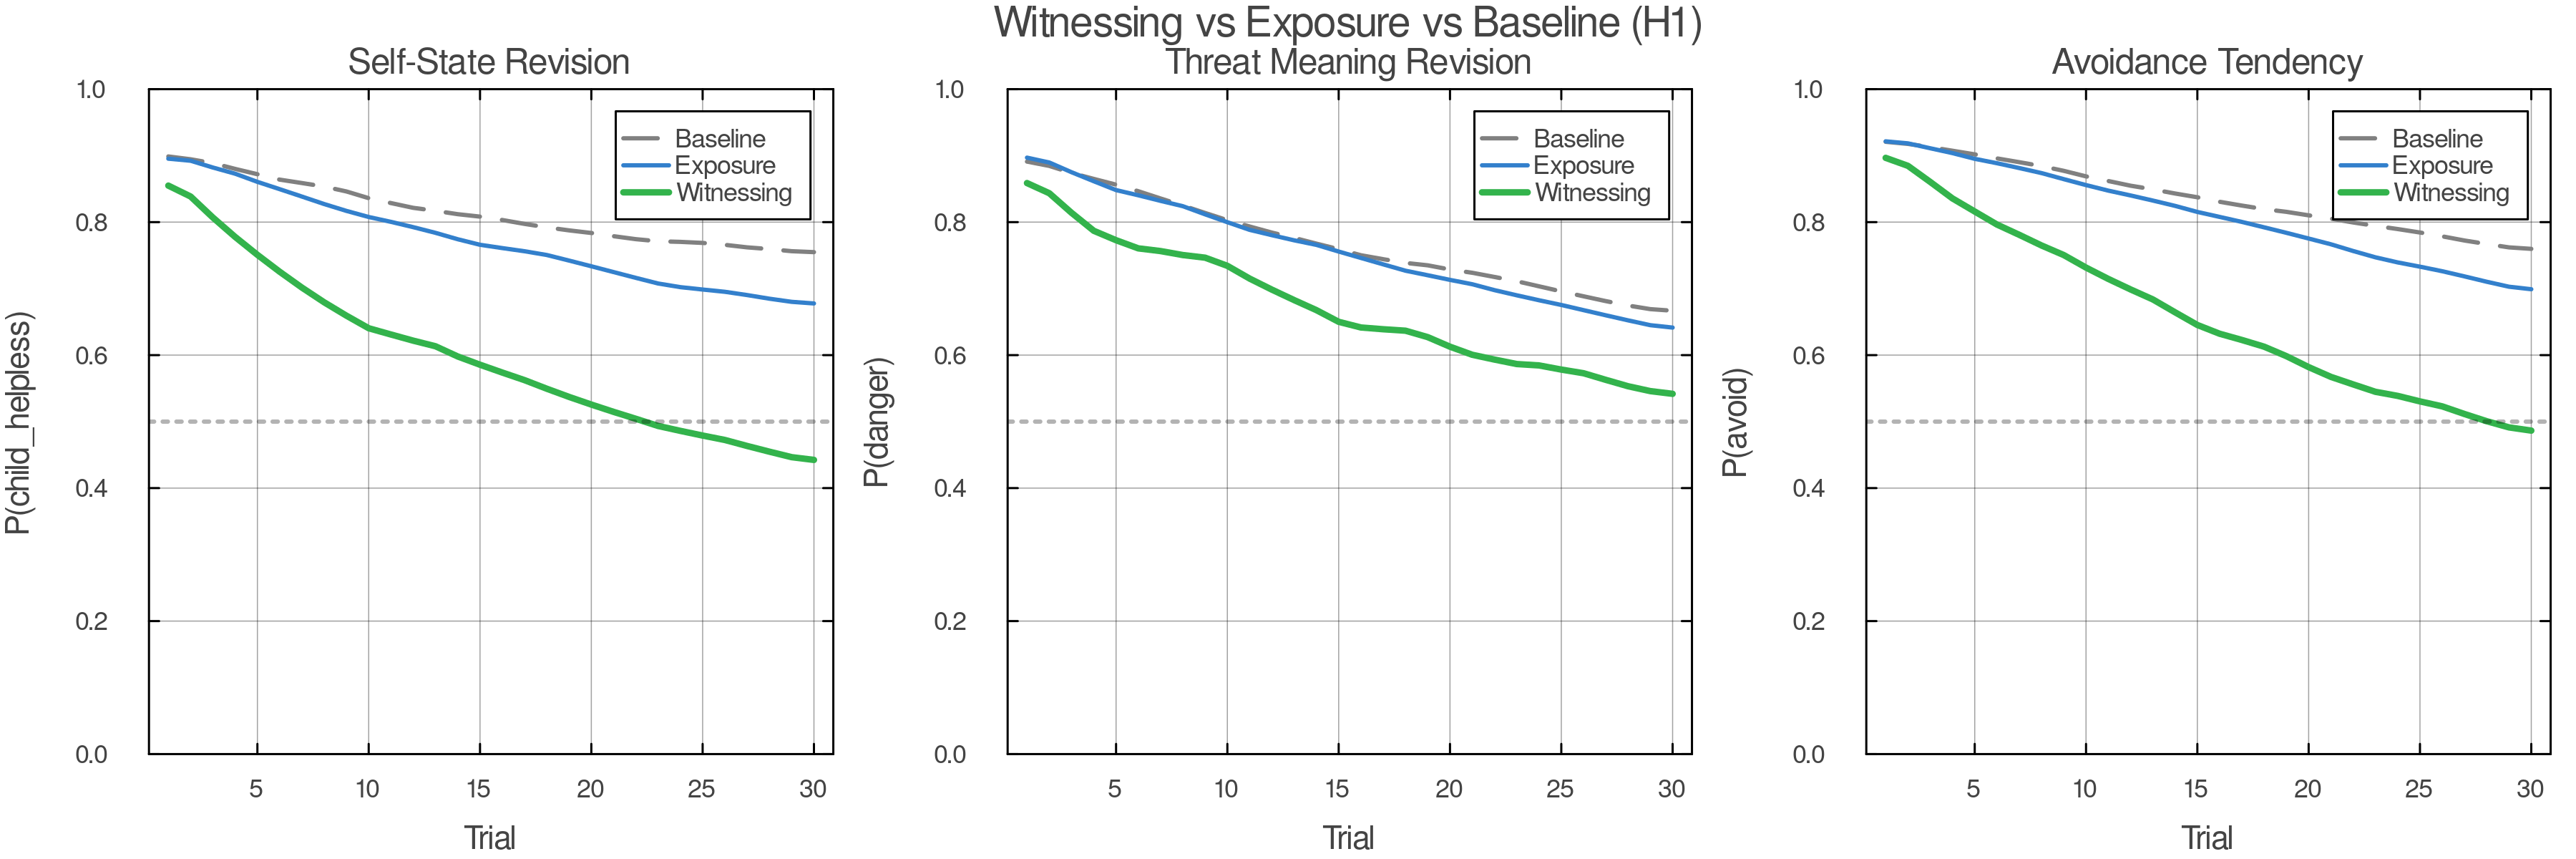
\includegraphics[width=0.96\linewidth]{fig2_witnessing_vs_exposure.png}
\caption{Witnessing versus exposure under matched activation. The model predicts broader and deeper change when context remains online under elevated Self-energy.}
\label{fig:witnessing-vs-exposure}
\end{figure}

Exposure (Condition 2) should show slower or weaker self-state revision
compared to witnessing (Condition 3), despite equivalent stimulus
contact. Threat meaning may update under exposure, but the change should
be narrower: specific to the trained stimulus rather than generalizing
to novel ambiguous-safe cues.

\subsection{13.4 Generalization}\label{generalization}

Witnessing should produce broader generalization to novel ambiguous-safe
cues than exposure. This follows from the H1 causal structure:
witnessing revises the upstream self-state prior, which cascades to
threat assessment across stimuli, while exposure revises specific
stimulus-threat associations.

\subsection{13.5 Real Danger
Preservation}\label{real-danger-preservation}

Under Condition 4, the model must preserve adaptive fear. Elevated
Self-energy should not flatten all threat responses. When the world is
actually dangerous, the system should correctly infer danger and select
protective policies. Witnessing enables discrimination, not suppression.

\subsection{13.6 Policy Ordering}\label{policy-ordering}

Under witnessing in the H1 model, policy change should lag self-state
change. Specifically, \(P(\text{avoid})\) should begin to decrease only
after \(P(s = \text{adult\_capable})\) has risen appreciably. This
temporal ordering is a distinctive prediction that differentiates the
model from accounts in which policy change and belief change are
contemporaneous.

\subsection{13.7 Partial Revision}\label{partial-revision-1}

Under brief or unstable witnessing windows --- where \(E_t\) is elevated
only transiently --- upstream priors should soften without fully
revising. The concentration parameters of the Dirichlet priors should
decrease (beliefs become less certain) without the mode shifting to
context-consistent values. This corresponds to the clinical observation
of partial unburdening.

\subsection{13.8 Model Comparison}\label{model-comparison}

\begin{figure}[htbp]
\centering
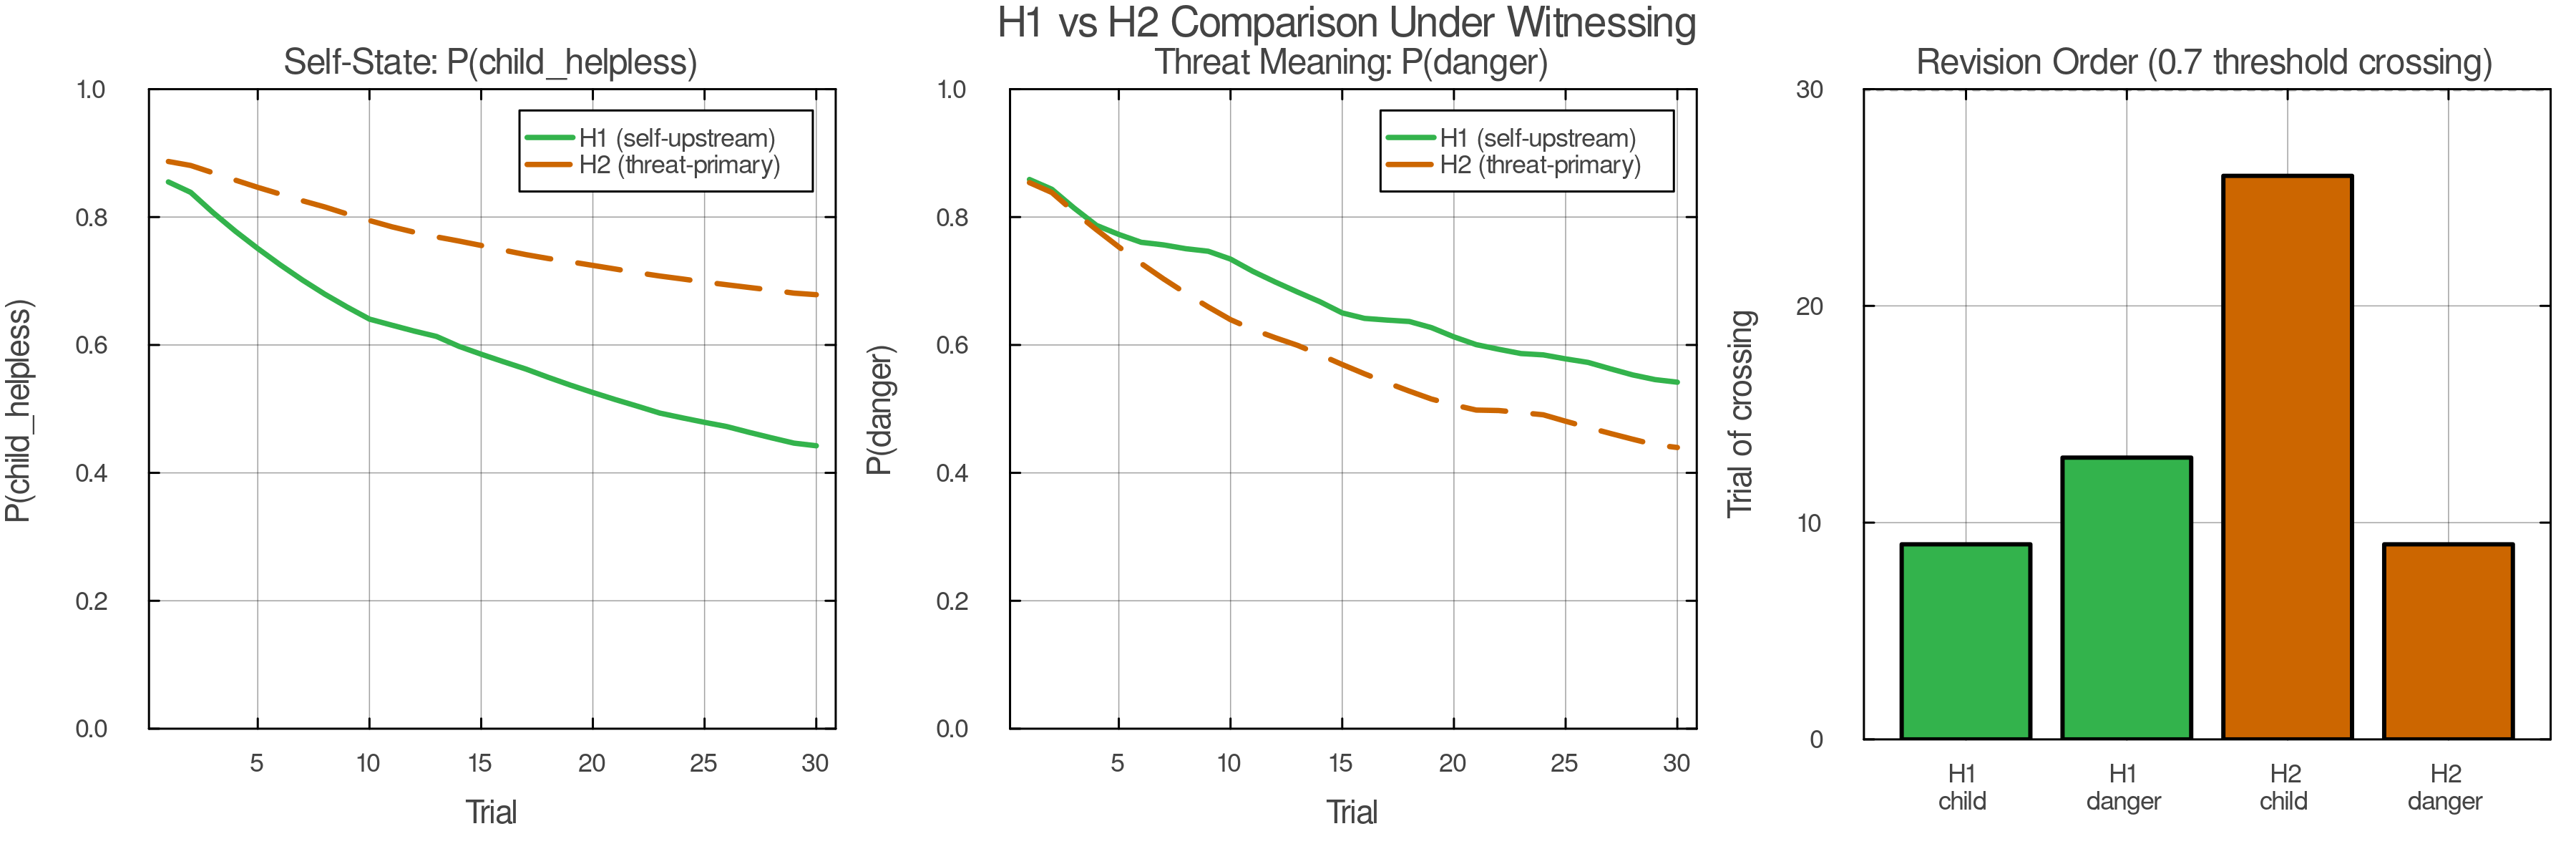
\includegraphics[width=0.96\linewidth]{fig3_h1_vs_h2_witnessing.png}
\caption{Model comparison for witnessing trajectories under H1 and H2. The self-state-upstream account predicts earlier self-state change and stronger generalization.}
\label{fig:h1-vs-h2}
\end{figure}

H1 should fit the resulting trajectories better than H2. Specifically,
H1 should produce: (a) earlier self-state revision under witnessing, (b)
a stronger generalization advantage, and (c) a temporal ordering in
which self-state change precedes threat meaning change. If H2 fits
equally well, the self-state-upstream hypothesis is weakened.

\subsection{13.9 Falsifiers}\label{falsifiers}

The proposed account is weakened if:

\begin{itemize}
\tightlist
\item
  High Self-energy does not change the relation to activation
\item
  Witnessing does not move self-state earlier than exposure
\item
  Exposure produces equal or better generalization
\item
  H2 fits as well as H1
\item
  Witnessing collapses fear globally, including in real danger
\item
  The dissociation control looks indistinguishable from witnessing
\end{itemize}

\section{14. Discussion}\label{discussion}

\subsection{14.1 What the Model Explains}\label{what-the-model-explains}

\begin{figure}[htbp]
\centering
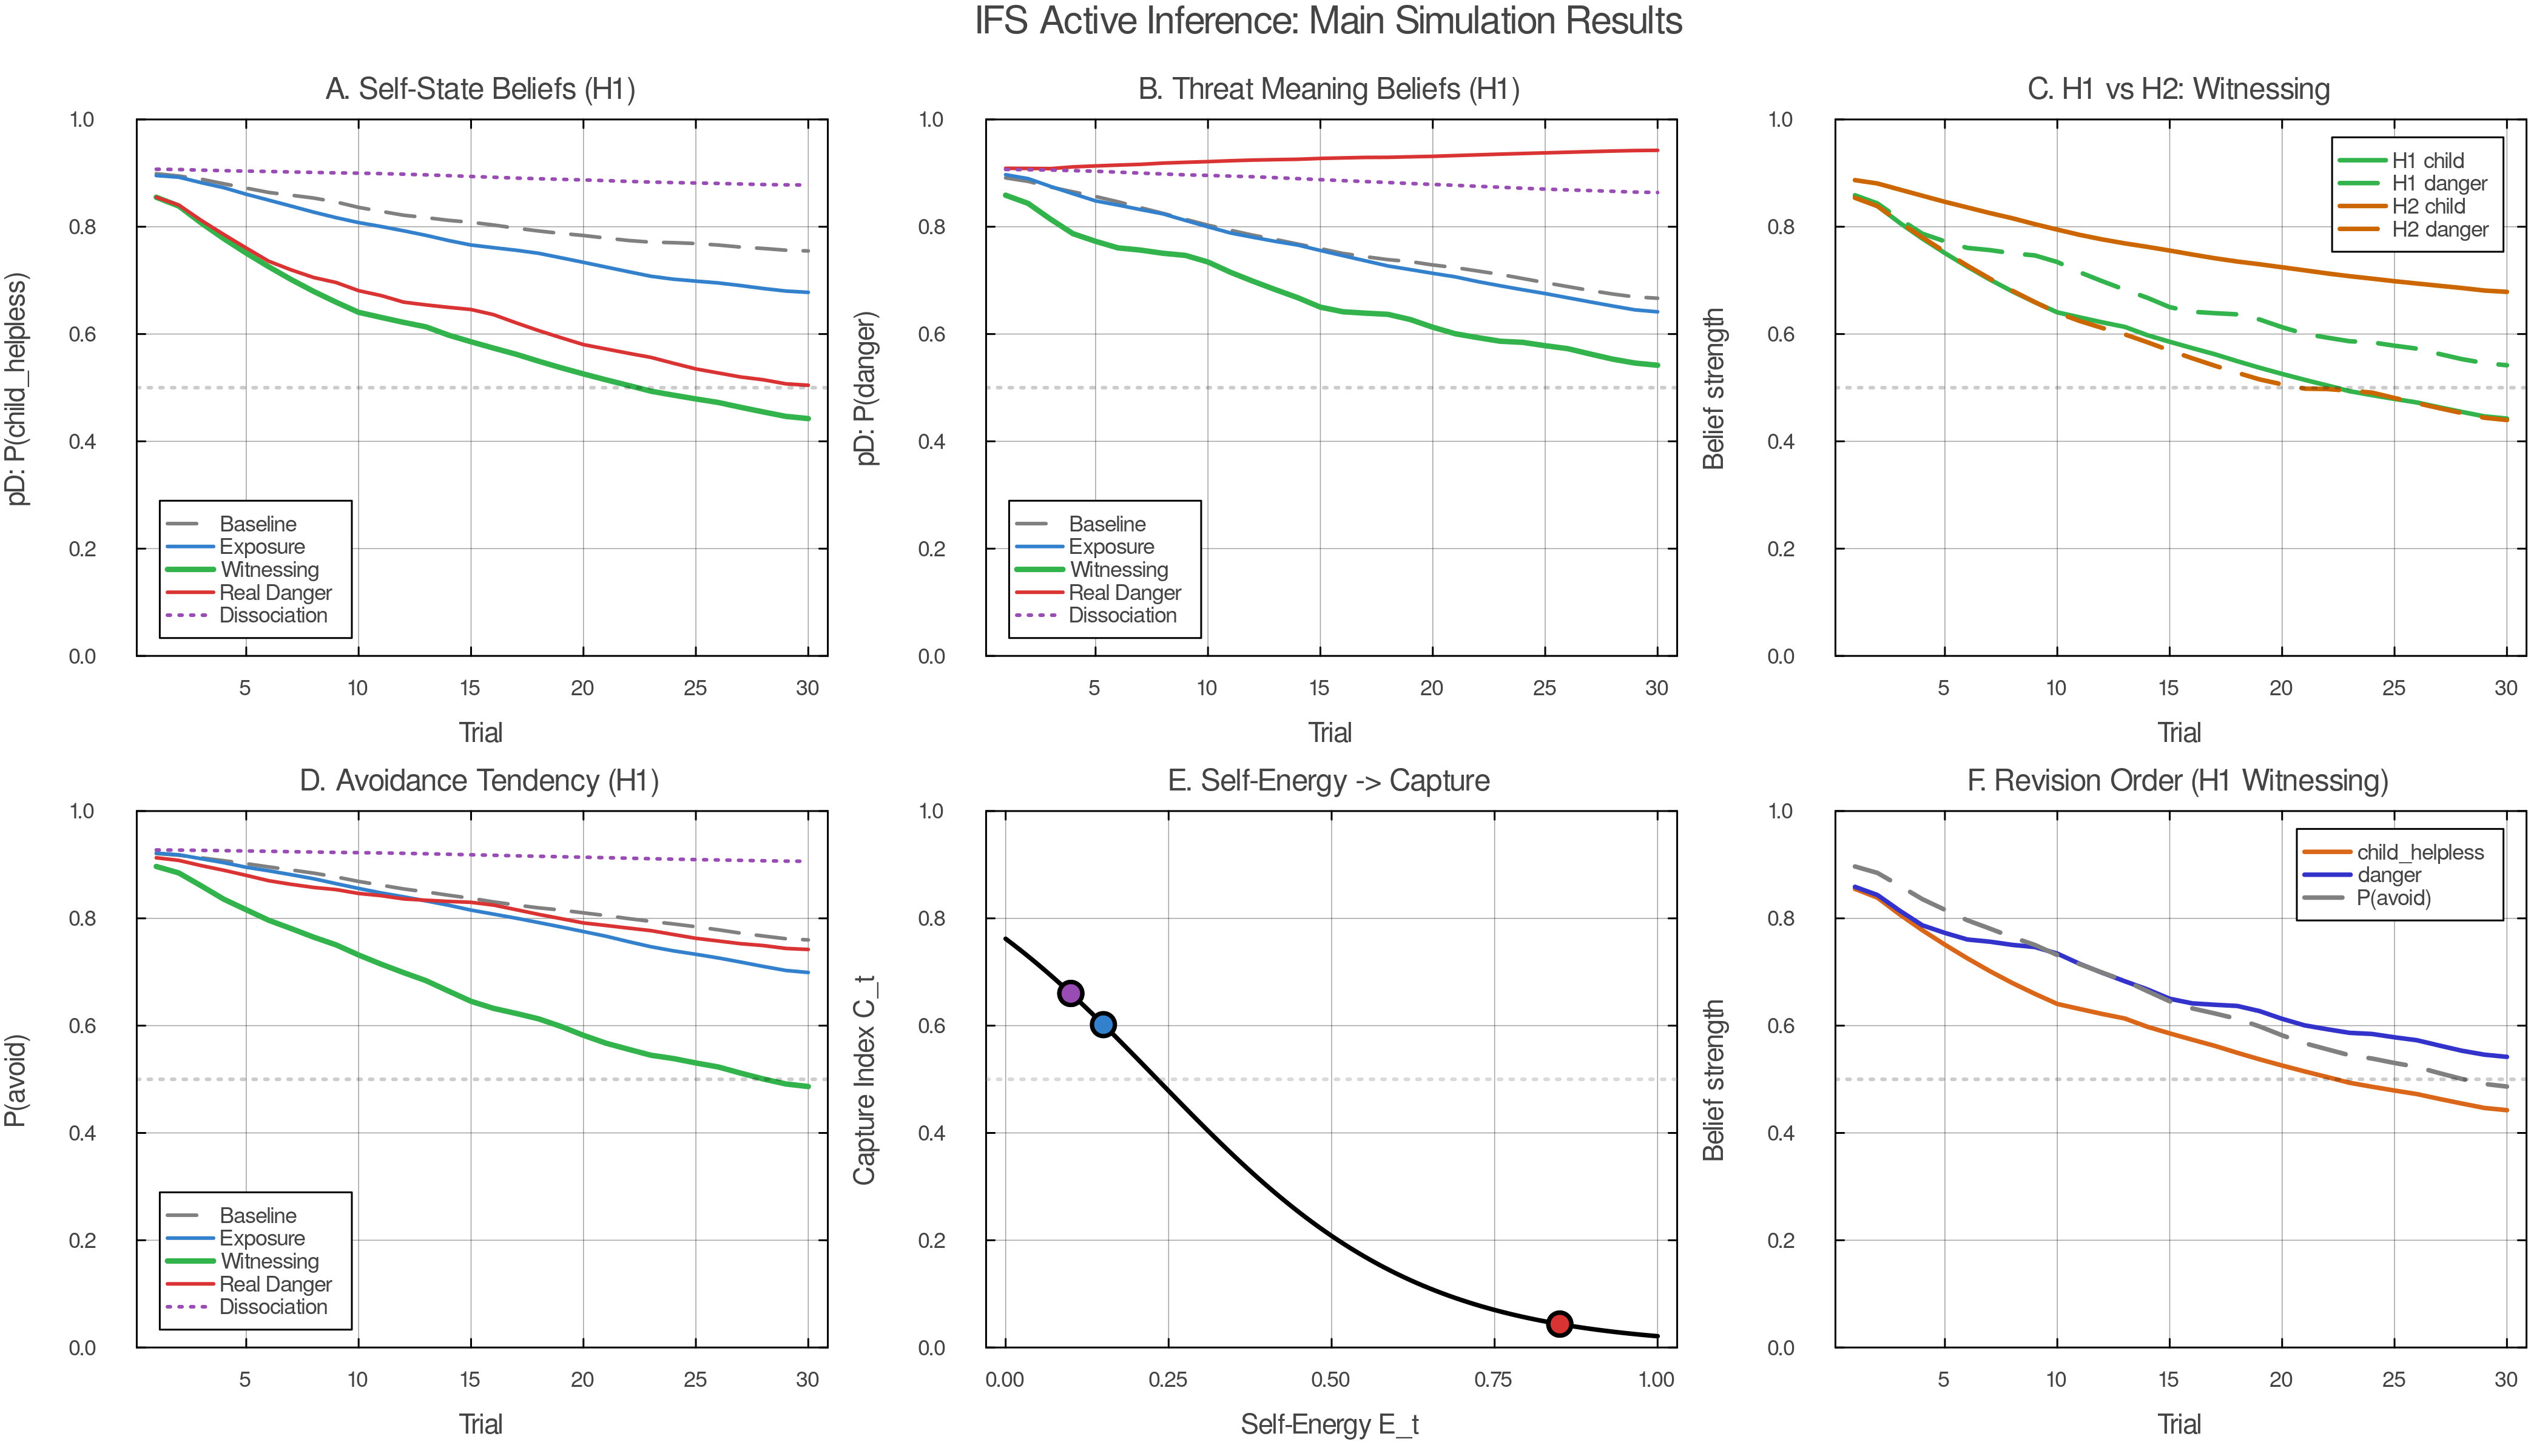
\includegraphics[width=0.96\linewidth]{fig7_main_summary.png}
\caption{Summary schematic of the paper's account: formation under threat plus low control, persistence through functional isolation, and revision through witnessing.}
\label{fig:main-summary}
\end{figure}

This paper argues that the central IFS question --- whether a part takes
over or is held in context --- can be formalized as a precision balance
between part priors and present-context evidence, governed by
Self-energy. The model makes specific, testable predictions about the
conditions under which change occurs, the order in which beliefs revise,
and the breadth of generalization.

The model counts as an IFS model despite being minimal --- addressing
single-part dynamics in a single-agent system --- because it captures
the core IFS distinction: the difference between being a part's beliefs
and being with a part's beliefs. That distinction, formalized through
the capture index, is what makes IFS therapeutically distinctive. The
phenomenological difference between ``I am afraid'' and ``a part of me
is afraid'' corresponds to a formal difference in precision regimes, and
the therapeutic consequence --- that only the second permits lasting
change --- follows from the model's structure.

\subsection{14.2 How the Model Differs from Related
Accounts}\label{how-the-model-differs-from-related-accounts}

\textbf{Exposure-based accounts} focus on activation and corrective
evidence. The present model agrees that both are necessary but argues
that a third variable --- Self-energy --- determines whether corrective
evidence can reach the beliefs that matter. Exposure revises
stimulus-threat associations; witnessing revises the upstream self-state
beliefs that generate threat assessments across stimuli.

\textbf{Schema-based accounts} (including Chamberlin's coherence therapy
model) identify modular or isolated belief structures as the target of
change. The present model agrees with the identification but proposes a
different mechanism of isolation: functional disconnection through
extreme prior precision rather than structural disconnection through
missing graph edges. This is not merely a notational preference; it
generates different predictions. Functional isolation predicts slow
updating under repeated safe exposure; structural isolation predicts
near-zero updating until reconnection. The clinical evidence suggests
both patterns exist, with functional isolation characterizing the more
common presentation.

\textbf{Self-energy differs from ordinary safety or calm.} Many
therapeutic approaches emphasize safety, and safety is important. But
safety alone does not predict the model's core phenomenon: that the same
activation under the same external conditions can produce either
blending or witnessing, depending on an internal variable. Self-energy
is composite --- involving both autonomic-social regulation and
metacognitive depth --- and it is this composite character that
distinguishes it from simple arousal reduction.

\subsection{14.3 Limitations}\label{limitations}

The model has several deliberate limitations that constrain its scope:

\textbf{The therapist is absent from the model.} The model describes
individual-level dynamics in what is, clinically, a deeply relational
process. Early in treatment, the therapist's Self-energy often supplies
the stability that the client cannot yet maintain alone. The present
model captures a minimal intra-agent mechanism but not the full dyadic
therapeutic field. The external support parameter \(u_t\) in the
simulation is a placeholder for what is, in practice, a rich
interpersonal process.

\textbf{Self-like parts are not distinguished from genuine Self.} The
model does not yet distinguish genuine witnessing from self-like
managerial imitation of witnessing. This is one of the most important
unresolved problems for a computational account of IFS, because apparent
metacognitive fluency is not always equivalent to genuine Self-ledness.
A self-like part may produce verbal reports of curiosity and compassion
while the underlying precision regime remains part-dominated.
Distinguishing these states computationally is a major target for future
work.

\textbf{Protector dynamics are simplified.} The model formalizes only
the minimum gatekeeping function of protectors. The full clinical
richness --- trust assessment, conditional permission, role
transformation, distinct manager and firefighter strategies --- awaits a
more complete multi-part model.

\textbf{The model operates at the algorithmic level.} No claims are made
about neural implementation. The mapping from precision regimes to
specific neural circuits --- likely involving prefrontal-limbic
interactions, vagal tone, and interoceptive processing networks --- is a
separate research program.

\subsection{14.4 Future Directions}\label{future-directions}

Several directions emerge naturally from the model's current
limitations:

\begin{enumerate}
\def\labelenumi{\arabic{enumi}.}
\item
  \textbf{Therapist as second agent.} Modeling the therapeutic
  relationship as a two-agent system in which the therapist's generative
  model interacts with the client's, providing external scaffolding for
  Self-energy.
\item
  \textbf{Self-like parts.} Formalizing the distinction between genuine
  witnessing (high V + high M) and pseudo-witnessing (high M alone, or
  high verbal reflection without embodied regulation). This may require
  separating the components of Self-energy in the simulation rather than
  using a scalar proxy.
\item
  \textbf{Multi-part parliament models.} Extending from single-part and
  two-part dynamics to the full clinical complexity of multiple
  interacting parts with heterogeneous roles.
\item
  \textbf{Empirical validation.} The model's predictions --- especially
  the temporal ordering of revision and the generalization advantage of
  witnessing over exposure --- are testable with existing clinical and
  neuroimaging methods.
\end{enumerate}

\section{Appendix A. Formation
Simulation}\label{appendix-a.-formation-simulation}

\subsection{A.1 Question}\label{a.1-question}

Can a part-like bundle form under overwhelm and low control without
invoking literal structural rewiring?

\subsection{A.2 Setup}\label{a.2-setup}

The simulation uses the same hidden variables as the main model: context
(\(c\)), self-state (\(s\)), and threat meaning (\(m\)). The agent
begins with relatively flat priors and low Self-energy.

\subsection{A.3 Acquisition Phase}\label{a.3-acquisition-phase}

\begin{figure}[htbp]
\centering
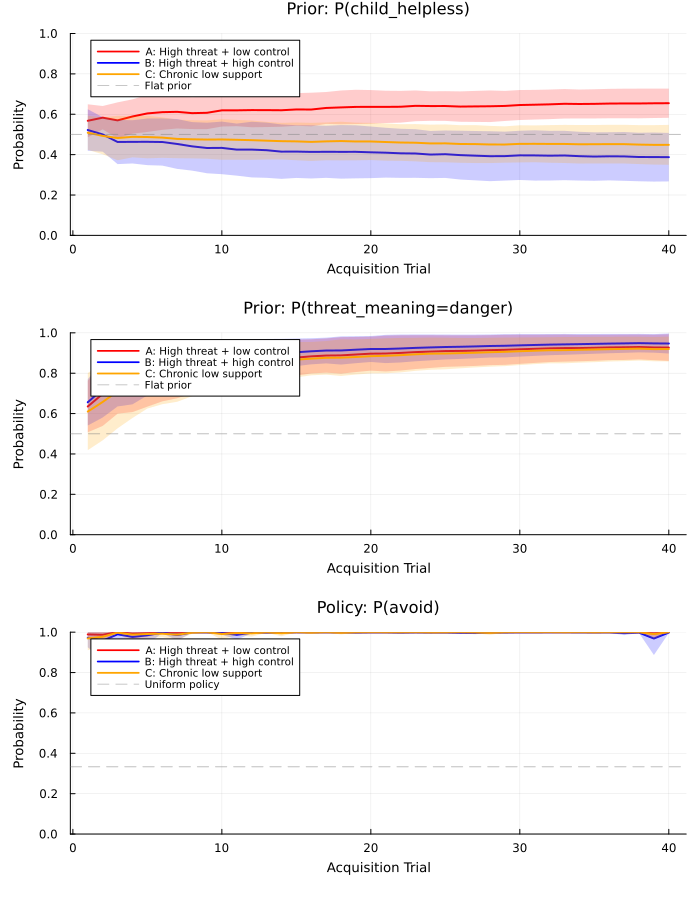
\includegraphics[width=0.96\linewidth]{formation_acquisition_trajectories.png}
\caption{Formation simulation acquisition trajectories across repeated episodes.}
\label{fig:formation-acquisition}
\end{figure}

The agent is exposed to repeated episodes with dangerous context,
ambiguous or threat-weighted cues, low support, and low controllability.
Avoidance succeeds in short-term error reduction; inspect and stay
policies fail or produce costly outcomes. Across episodes, the agent's
priors on \(s = \text{child\_helpless}\), \(m = \text{danger}\), and
\(\pi_{\text{avoid}}\) should strengthen through Dirichlet learning.

\subsection{A.4 Controllability
Gradient}\label{a.4-controllability-gradient}

\begin{figure}[htbp]
\centering
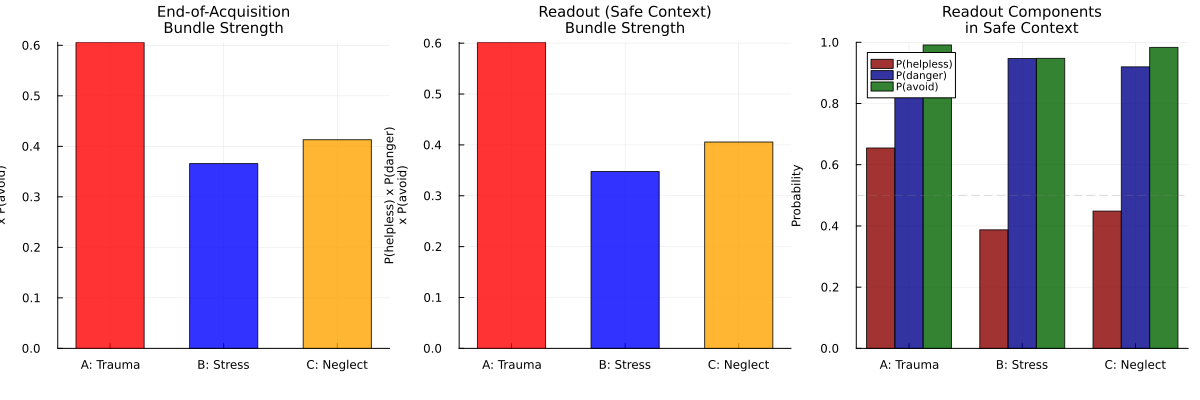
\includegraphics[width=0.96\linewidth]{formation_controllability_gradient.png}
\caption{Controllability gradient in the formation simulation. Low control under threat produces stronger part-like bundle acquisition than threat alone.}
\label{fig:formation-controllability}
\end{figure}

The simulation compares at least two conditions:

\textbf{Condition A (high threat + low control):} Classic acute trauma
formation. The agent has little influence over outcomes; avoidance is
the only reliably cost-reducing policy.

\textbf{Condition B (high threat + high control):} Frightening but
manageable. The agent can select inspect or stay and receive neutral or
positive outcomes. This condition should be distressing but not
part-forming.

\textbf{Condition C (optional --- moderate chronic threat + chronic low
support):} Neglect-like formation. Lower acute threat but sustained low
control and absence of support. Formation may be slower but should still
occur.

\subsection{A.5 Main Prediction}\label{a.5-main-prediction}

\begin{figure}[htbp]
\centering
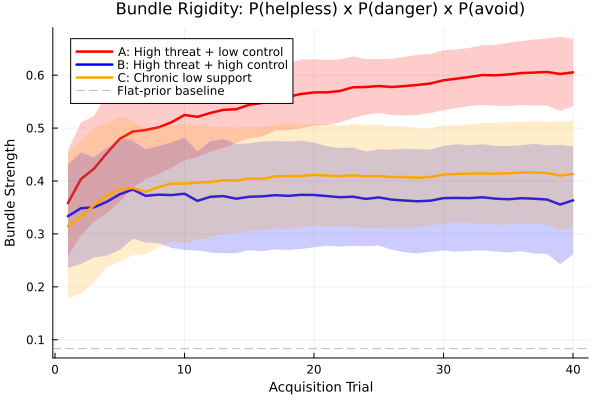
\includegraphics[width=0.96\linewidth]{formation_bundle_rigidity.png}
\caption{Bundle rigidity as a function of helplessness during formation. More severe low-control conditions produce more treatment-resistant priors.}
\label{fig:formation-rigidity}
\end{figure}

Formation depends more strongly on low control under threat than on
threat alone. Condition A should produce rigid bundles; Condition B
should not; Condition C (if included) should produce bundles with
different characteristics --- slower formation, potentially different
rigidity profiles.

The model also predicts that degree of helplessness should scale bundle
rigidity: more severe low-control conditions produce more
treatment-resistant prior bundles.

\subsection{A.6 Readout}\label{a.6-readout}

\begin{figure}[htbp]
\centering
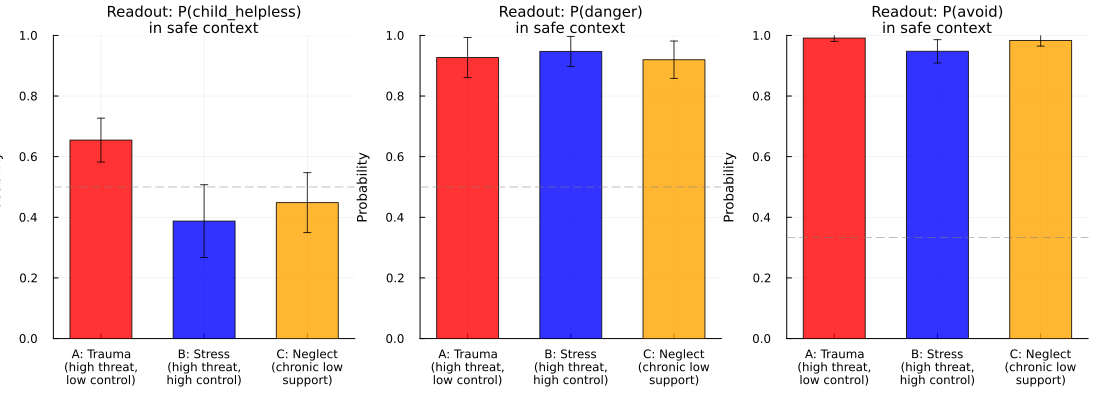
\includegraphics[width=0.96\linewidth]{formation_readout_comparison.png}
\caption{Post-acquisition readout in a safe ambiguous context. Formed bundles over-infer helplessness, danger, and avoidance despite safety.}
\label{fig:formation-readout}
\end{figure}

After acquisition, the agent is placed in a safe, ambiguous context. If
formation occurred, the agent should infer helplessness too readily,
infer danger too readily, and avoid despite safety --- demonstrating
that a part-like bundle has formed through precision-based learning
without explicit structural rewiring.

\section{Appendix B. Polarization
Simulation}\label{appendix-b.-polarization-simulation}

\subsection{B.1 Question}\label{b.1-question}

How does the model explain multi-part polarization and its
phenomenology, and how does Self-energy modulate the dynamics?

\subsection{B.2 Setup}\label{b.2-setup}

Introduce two part-bundles with opposing preferred policies:

\begin{itemize}
\tightlist
\item
  \textbf{Part A} (approach / attach / disclose): priors favoring
  connection.
\item
  \textbf{Part B} (withdraw / protect / avoid): priors favoring safety
  through distance.
\end{itemize}

Each bundle includes self-state, world-state, preferred policy, expected
outcome, and --- critically --- a threat estimate about the other
bundle's policy.

\subsection{B.3 Dynamics}\label{b.3-dynamics}

\begin{figure}[htbp]
\centering
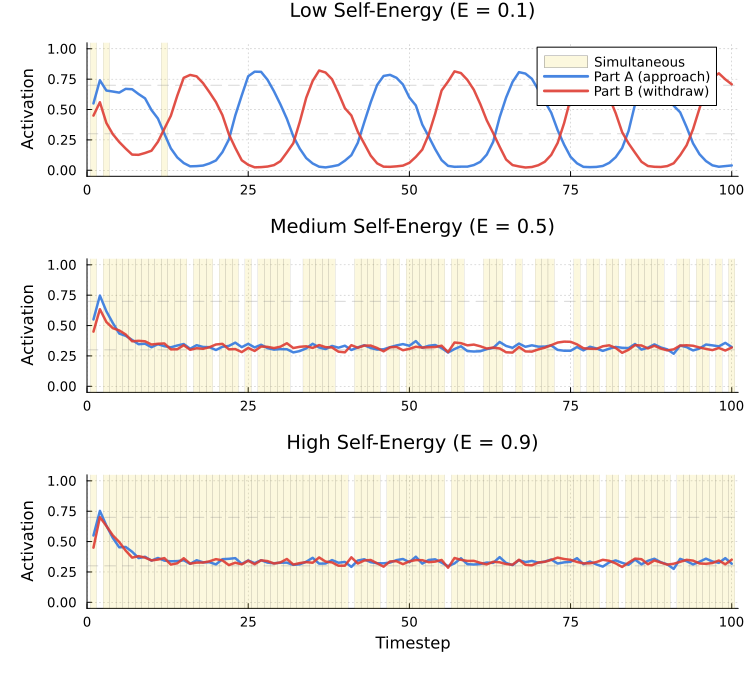
\includegraphics[width=0.96\linewidth]{polarization_timeseries.png}
\caption{Polarization dynamics under mutual threat modeling. Low Self-energy yields anti-phase switching between competing parts.}
\label{fig:polarization-timeseries}
\end{figure}

Under low Self-energy, mutual threat modeling produces anti-phase
oscillation:

\[a_{A,t+1} = \sigma(\theta_A \cdot \text{cue}_A + \kappa_A \cdot \mathbb{1}[\text{action}_{B,t}] - \eta E_t)\]
\[a_{B,t+1} = \sigma(\theta_B \cdot \text{cue}_B + \kappa_B \cdot \mathbb{1}[\text{action}_{A,t}] - \eta E_t)\]

where \(\kappa_A, \kappa_B > 0\) encode mutual threat assessment and
higher \(E_t\) dampens takeover dynamics.

\subsection{B.4 Predicted
Phenomenology}\label{b.4-predicted-phenomenology}

\begin{figure}[htbp]
\centering
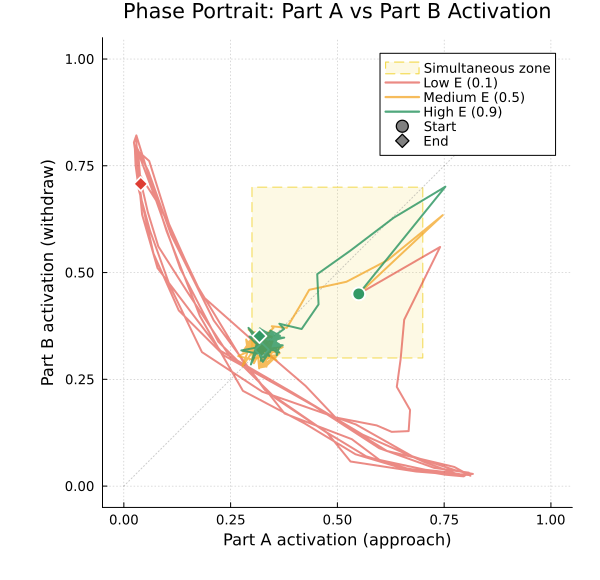
\includegraphics[width=0.96\linewidth]{polarization_phase.png}
\caption{Phase portrait of competing part activations under lower and higher Self-energy.}
\label{fig:polarization-phase}
\end{figure}

\textbf{Low Self-energy:} Rapid reversals, unstable commitments, ``both
feel true but not at the same time,'' exhaustion from oscillation.

\textbf{Higher Self-energy:} Both bundles can be represented without
either capturing inference. Oscillation dampens. Mixed or negotiated
policies become available. The contradiction becomes observable rather
than identity-level.

\subsection{B.5 Dependent Measures}\label{b.5-dependent-measures}

\begin{figure}[htbp]
\centering
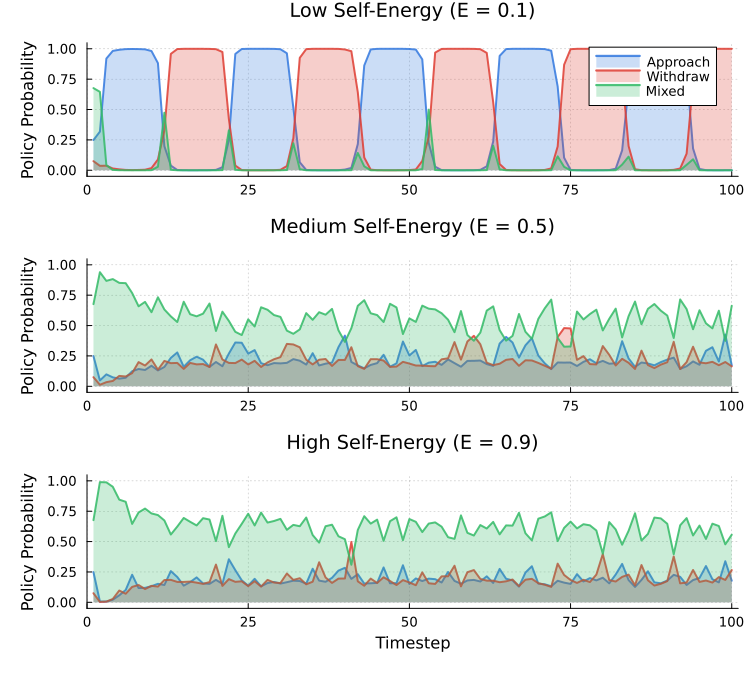
\includegraphics[width=0.96\linewidth]{polarization_policy.png}
\caption{Policy selection across polarization dynamics as Self-energy changes.}
\label{fig:polarization-policy}
\end{figure}

\begin{figure}[htbp]
\centering
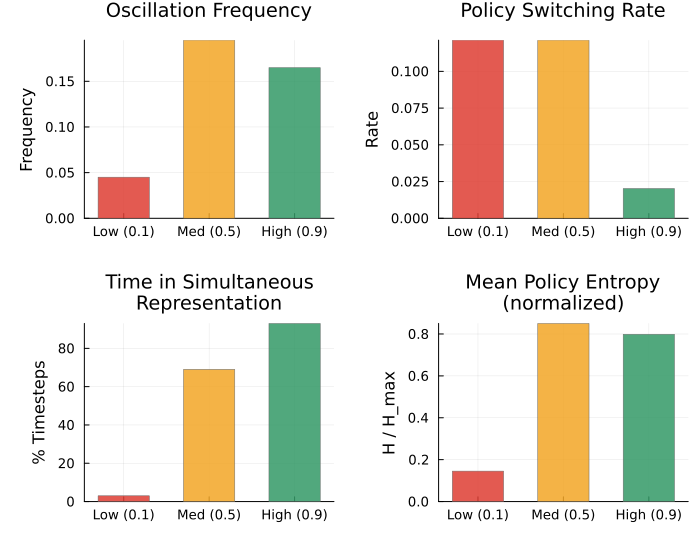
\includegraphics[width=0.96\linewidth]{polarization_summary.png}
\caption{Summary measures for oscillation, switching, entropy, and simultaneous representation in the polarization simulation.}
\label{fig:polarization-summary}
\end{figure}

\begin{figure}[htbp]
\centering
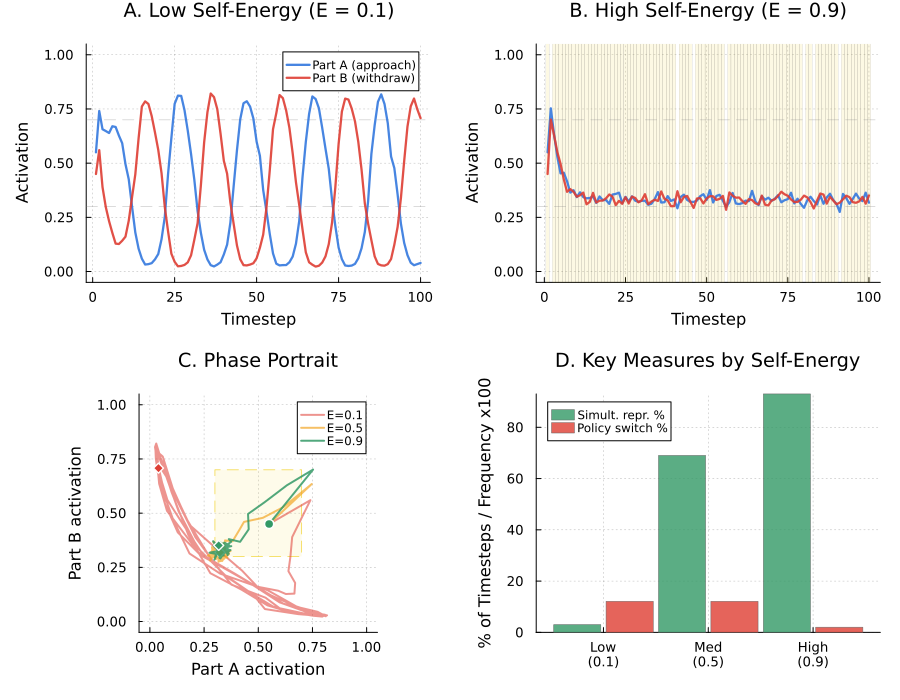
\includegraphics[width=0.96\linewidth]{polarization_combined.png}
\caption{Combined polarization results, integrating dynamic and summary views of de-polarization under higher Self-energy.}
\label{fig:polarization-combined}
\end{figure}

\begin{itemize}
\tightlist
\item
  Oscillation frequency
\item
  Switching rate between dominant parts
\item
  Part activation anti-correlation
\item
  Policy entropy
\item
  Duration of mixed-policy stability as Self-energy increases
\item
  \textbf{Time spent in simultaneous representation without takeover}
  --- both parts active, neither dominating
\item
  \textbf{Time to negotiated policy emergence} --- first trial where the
  selected policy is not the preferred policy of either dominant part
\end{itemize}

These last two measures are closest to clinical relevance: the
transition from ``stuck oscillation'' to ``both perspectives held, new
possibility available.''

\section{References}\label{references}

{[}TODO --- to be compiled during final assembly{]}
\end{document}
